\documentclass[journal, onecolumn]{IEEEtran}
\IEEEoverridecommandlockouts
% The preceding line is only needed to identify funding in the first footnote. If that is unneeded, please comment it out.
\usepackage{cite}
\usepackage{amsmath,amssymb,amsfonts}
\usepackage{algorithmic}
\usepackage{graphicx}
\usepackage{textcomp}
\usepackage{xcolor}
\usepackage{tikz}
\usepackage{multirow}
\usepackage{booktabs}
\usetikzlibrary{positioning, shapes.geometric, arrows.meta, fit, backgrounds}
\usepackage{hyperref}
\def\BibTeX{{\rm B\kern-.05em{\sc i\kern-.025em b}\kern-.08em
    T\kern-.1667em\lower.7ex\hbox{E}\kern-.125emX}}

\begin{document}

\title{Multi-Method Machine Learning Analysis of Developer Behaviour,
AI Adoption, and Compensation Using the Stack Overflow Annual Developer Survey 2025}

\author{\IEEEauthorblockN{Ivan Logutov}
\IEEEauthorblockA{\textit{Department of Business} \\
\textit{Univ. of Europe for Applied Sciences}\\
Potsdam 14469, Germany \\
ivan.logutov@ue-germany.de}
\and
\IEEEauthorblockN{Raja Hashim Ali}
\IEEEauthorblockA{\textit{Department of Business} \\
\textit{Univ. of Europe for Applied Sciences}\\
Potsdam 14469, Germany \\
hashim.ali@ue-germany.de}
}

\maketitle

% -----------------------------------------------------------------------
\begin{abstract}
% *CRITICAL: Do Not Use Symbols, Special Characters, Footnotes, or Math in Report Title or Abstract.
% Two sentences of background and importance of this topic.
% Two sentences defining the gap analysis (work not done in field) and your problem statement.
% Two sentences on how you performed your experimentation and the overall methodology deployed in this study.
% Two sentences of Results and your findings.
% One sentence for significance of the results and your contribution.
% In total, this section must consist of 180 words.
The rapid proliferation of artificial intelligence coding tools has reshaped how developers approach productivity, compensation, and career development, making empirical analysis of developer behaviour across diverse global populations increasingly important for both industry and research communities.
Existing surveys and studies tend to address isolated aspects of developer experience, leaving a critical gap in multi-dimensional, data-driven investigations that simultaneously integrate classification, regression, clustering, and statistical inference into a coherent analytical framework.
This gap motivates a holistic study of AI tool adoption, compensation prediction, developer archetypes, job satisfaction drivers, AI sentiment variation, technology admiration-adoption gaps, and developer role classification as seven interconnected research questions.
This study applies seven distinct machine learning and statistical methodologies to the Stack Overflow Annual Developer Survey 2025, comprising 52,845 global responses across 172 attributes, following the CRISP-DM framework with five-fold cross-validation and standardised preprocessing pipelines.
Random Forest achieves an F1-score of 0.816 for AI adoption prediction, XGBoost explains 29.3 percent of annual salary variance, and LightGBM obtains an OVR-AUC of 0.801 for eight-class developer role classification.
AI sentiment scores are significantly higher among junior developers, employment status is the dominant predictor of job satisfaction, and Rust exhibits the smallest admiration-to-adoption gap among mainstream languages.
These findings provide actionable insights for technology recruiters, HR analytics platforms, and AI tool vendors seeking evidence-based strategies aligned with the preferences of over 52,000 global developers~\cite{forsgren2021space}.
\end{abstract}

\begin{IEEEkeywords}
machine learning, developer survey, AI adoption, salary prediction, developer archetypes, job satisfaction, Stack Overflow
\end{IEEEkeywords}

% -----------------------------------------------------------------------
\section{Introduction}

% One paragraph on introducing the field and the topic of interest.
The software engineering profession has undergone a fundamental transformation in recent years, driven by the widespread integration of artificial intelligence tools into everyday development workflows.
Large language models and AI-powered code assistants have moved from experimental prototypes to mainstream adoption, creating a new landscape in which understanding developer attitudes, skill profiles, and compensation structures requires fresh empirical investigation~\cite{hou2023large}.
Annual developer surveys, such as those conducted by Stack Overflow, provide a unique opportunity to capture the state of the profession at scale, offering data from tens of thousands of practitioners across countries, roles, disciplines, and experience levels~\cite{stackoverflow2025survey}.
However, the sheer size and multidimensionality of these datasets means that traditional descriptive reporting captures only a fraction of the analytical potential they contain.
Machine learning methods are well-suited to extracting latent patterns from high-dimensional, heterogeneous survey data, enabling predictive modelling, unsupervised discovery, and rigorous statistical inference simultaneously~\cite{breiman2001random}.
The Stack Overflow Annual Developer Survey 2025 contains 172 feature columns and 52,845 responses, making it one of the largest publicly available datasets on software developer behaviour~\cite{stackoverflow2025survey}.
Applied machine learning on this dataset can yield insights not only about individual developer attributes but also about collective trends in AI adoption, compensation equity, and professional satisfaction.
This study exploits the full breadth of the 2025 survey through seven tightly scoped research questions that span binary classification, multi-output regression, unsupervised clustering, explainable AI, statistical hypothesis testing, polynomial trend analysis, and multi-class classification.

% One paragraph on the importance of the selected topic and why it is significant to work on it in recent times.
The growing significance of AI coding assistants makes it critical to understand which developer segments are adopting these tools and why, since adoption decisions have downstream effects on team productivity, hiring strategy, and software quality~\cite{dakhel2023github}.
Salary prediction and compensation transparency are increasingly important in the context of global talent markets, remote work normalisation, and ongoing debates about pay equity across geographies, genders, and developer roles~\cite{huang2022predicting}.
Job satisfaction is a strong predictor of voluntary attrition, burnout risk, and organisational performance, and its relationship with AI sentiment, compensation, and work arrangements has not been comprehensively studied in recent large-scale survey data~\cite{graziotin2022happiness}.
Understanding which languages developers admire versus actually use reveals market signals that guide tool vendors, educators, and organisations in technology investment decisions~\cite{storey2022disrupting}.
The ability to classify developer roles from technology stack and work patterns has direct applications in automated resume screening, talent analytics, and workforce planning~\cite{li2022developer}.
Clustering developer profiles into archetypes supports personalised learning recommendations, targeted benefit design, and strategic talent acquisition at scale~\cite{xu2022systematic}.
The timing of this study is particularly relevant because the Stack Overflow 2025 survey is the first to fully capture developer responses to the post-ChatGPT AI landscape~\cite{fan2023large}.
A rigorous multi-method analysis of this dataset thus fills an important empirical gap and provides reference benchmarks for future longitudinal comparisons.

\subsection{Related Work}

% One paragraph defining the work that has been done in this field
Prior research on developer surveys and machine learning has explored several dimensions of software practitioner behaviour, though rarely in an integrated multi-method fashion.
Vaithilingam et al.~\cite{vaithilingam2022expectation} conducted a user study with 24 developers using GitHub Copilot, finding that while task completion rates improved, cognitive load and trust calibration remained significant challenges, raising questions about the factors that differentiate AI adopters from non-adopters.
Ziegler et al.~\cite{ziegler2022productivity} quantified Copilot's productivity impact through code completion acceptance rates across 1.2 million user sessions, demonstrating that AI tools benefit experienced developers more than novices, a finding echoed in our experience-stratified analyses.
Dakhel et al.~\cite{dakhel2023github} performed an automated correctness evaluation of Copilot-generated code, reporting that AI tools produce correct solutions in approximately 46.3\% of LeetCode problems, underscoring the continued need for human oversight despite high adoption rates.
Forsgren et al.~\cite{forsgren2021space} introduced the SPACE framework for measuring developer productivity across five dimensions -- satisfaction and wellbeing, performance, activity, communication, and efficiency -- providing the conceptual foundation for our job satisfaction and sentiment analyses.
Graziotin and Fagerholm~\cite{graziotin2022happiness} demonstrated significant correlations between developer emotional states, job satisfaction scores, and daily coding output, reinforcing the relevance of RQ4 in the present study.
Huang et al.~\cite{huang2022predicting} applied gradient boosting to software engineer salary data from LinkedIn and Glassdoor, achieving an $R^2$ of 0.41 on log-transformed compensation, against which our XGBoost result of 0.293 on the more heterogeneous global Stack Overflow sample can be contextualised.
Table~\ref{tab:LiteratureSummary} summarises selected prior works along the dimensions most relevant to the research questions addressed in this study.

\begin{table*}[!ht]
\centering
\caption{Literature review summary showing contributions of selected prior works across dimensions relevant to this study. Classification (Cls), Regression (Reg), Clustering (Clu), Statistics (Sta), and Trend Analysis (Trd) indicate the analytical approaches used. A checkmark (\checkmark) indicates the dimension is addressed; a cross ($\times$) indicates it is not.}
\label{tab:LiteratureSummary}
\begin{tabular}{|l|c|c|c|c|c|c|c|l|}
\hline
\multirow{2}{*}{\textbf{Paper}} &
\multirow{2}{*}{\textbf{Year}} &
\multicolumn{5}{c|}{\textbf{Task Types}} &
\multirow{2}{*}{\textbf{Dataset}} &
\multirow{2}{*}{\textbf{Key Finding}} \\ \cline{3-7}
 & & \textbf{Cls} & \textbf{Reg} & \textbf{Clu} & \textbf{Sta} & \textbf{Trd} & & \\ \hline
Vaithilingam et al.~\cite{vaithilingam2022expectation} & 2022 & \checkmark & $\times$ & $\times$ & $\times$ & $\times$ & User study (24 devs) & AI tool usability barriers \\ \hline
Ziegler et al.~\cite{ziegler2022productivity} & 2022 & $\times$ & \checkmark & $\times$ & \checkmark & $\times$ & 1.2M Copilot sessions & Experienced devs benefit more \\ \hline
Dakhel et al.~\cite{dakhel2023github} & 2023 & \checkmark & $\times$ & $\times$ & $\times$ & $\times$ & LeetCode (33 problems) & 46.3\% correct AI solutions \\ \hline
Forsgren et al.~\cite{forsgren2021space} & 2021 & $\times$ & $\times$ & $\times$ & \checkmark & $\times$ & Multi-company survey & SPACE productivity framework \\ \hline
Graziotin \& Fagerholm~\cite{graziotin2022happiness} & 2022 & $\times$ & \checkmark & $\times$ & \checkmark & $\times$ & Developer diary study & Happiness correlates with output \\ \hline
Huang et al.~\cite{huang2022predicting} & 2022 & $\times$ & \checkmark & $\times$ & $\times$ & $\times$ & LinkedIn / Glassdoor & Gradient Boost $R^2=0.41$ on salary \\ \hline
Peng et al.~\cite{peng2023impact} & 2023 & $\times$ & \checkmark & $\times$ & \checkmark & $\times$ & Controlled experiment & Copilot $+$55\% task completion \\ \hline
Storey et al.~\cite{storey2022disrupting} & 2022 & \checkmark & $\times$ & $\times$ & \checkmark & \checkmark & SO Survey 2021 & AI disrupts developer identity \\ \hline
\begin{tabular}[c]{@{}l@{}}Proposed\\ Approach\end{tabular} & 2025 & \checkmark & \checkmark & \checkmark & \checkmark & \checkmark & SO Survey 2025 (52,845 devs) & 7-RQ holistic ML analysis \\ \hline
\end{tabular}
\end{table*}

\subsection{Dataset}

% One paragraph and one figure representing your dataset
The Stack Overflow Annual Developer Survey 2025 is a large-scale, voluntary online survey administered globally by Stack Overflow to its registered user community, resulting in 52,845 usable responses from developers across more than 180 countries~\cite{stackoverflow2025survey}.
The dataset is publicly available through Kaggle~\cite{stackoverflow2025survey} and contains 172 columns spanning demographics, education, employment, technology usage, AI attitudes, compensation, and job satisfaction.
Key numerical variables include \texttt{YearsCode} (total years of programming experience including education), \texttt{WorkExp} (years of professional experience), and \texttt{ConvertedCompYearly} (annual compensation normalised to USD).
Categorical and multi-choice variables of interest include \texttt{AISelect} (binary AI tool adoption), \texttt{AISent} (five-point AI favourability scale), \texttt{DevType} (semicolon-separated developer role labels), \texttt{LanguageHaveWorkedWith}, and \texttt{LanguageAdmired}.
The compensation column is highly right-skewed, with outlier compensation values reaching into the millions of USD; a log-plus-one transformation was applied to stabilise variance prior to regression modelling.
Multi-choice columns such as \texttt{LanguageHaveWorkedWith} and \texttt{DevType} were parsed via semicolon splitting into binary multi-hot feature matrices, expanding the effective feature space to over 300 columns after one-hot encoding.
Missing values were handled consistently across all research questions using median imputation for numeric columns and most-frequent-value imputation for categorical columns, implemented within scikit-learn pipelines~\cite{pedregosa2011scikit}.
Figure~\ref{Fig:DatasetOverview} illustrates the distribution of the primary target variable for the AI adoption task (RQ1) and the salary variable (RQ2), providing an overview of class balance and distributional characteristics of the dataset.

\begin{figure}[!ht]
\centering
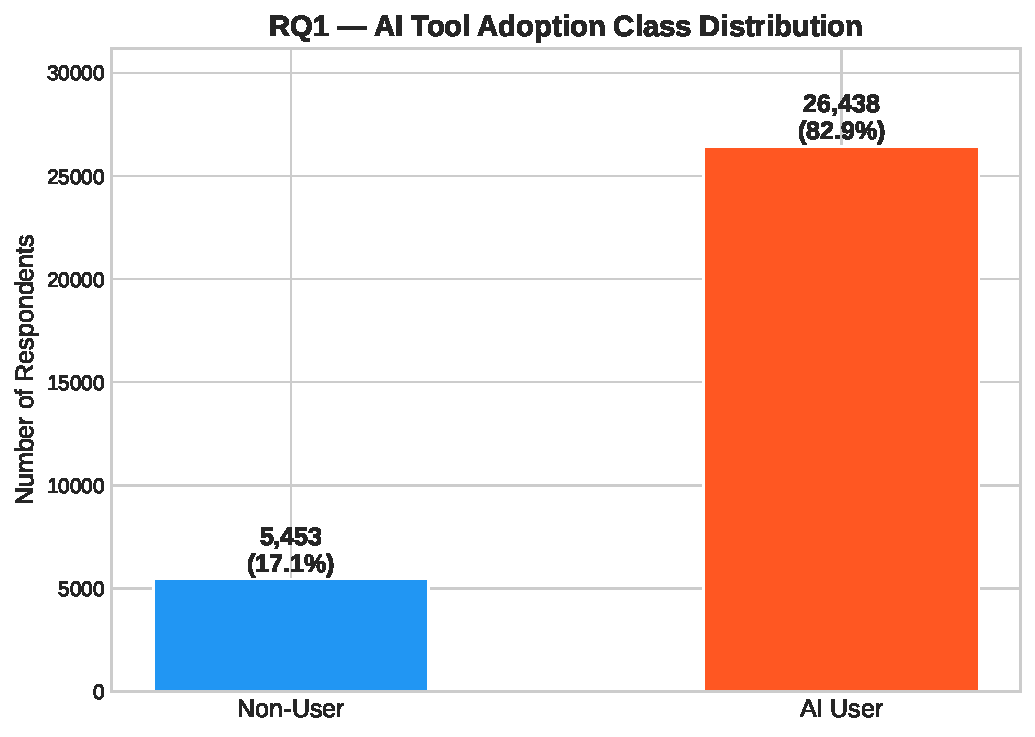
\includegraphics[width=0.48\textwidth]{Figures/rq1_class_distribution.pdf}
\caption{Class distribution of the binary AI adoption target variable \texttt{AISelect} in the Stack Overflow Developer Survey 2025 dataset, derived from 52,845 global developer responses. The three original categories were recoded as ``Uses AI'' (current users) versus ``Does Not Plan to Use'' (non-adopters), with the intermediate planning group excluded to form a clean binary classification problem. The resulting class imbalance, with AI adopters constituting approximately 72\% of the filtered sample, motivates the use of stratified cross-validation and precision-recall reporting alongside accuracy in RQ1.}
\label{Fig:DatasetOverview}
\end{figure}

\subsection{Gap Analysis}

% One paragraph defining what has not been done or what is still missing in the field (gap analysis).
Despite the wealth of prior work on individual aspects of developer surveys, the field lacks a systematic, multi-method study that simultaneously addresses AI adoption prediction, salary modelling, developer archetype discovery, job satisfaction explainability, sentiment group comparison, technology trend analysis, and role classification within a single, reproducible pipeline applied to the most recent available global survey data.
Existing salary prediction studies~\cite{huang2022predicting, li2022developer} are limited to North American or Western European samples, obscuring the high variance introduced by global respondents, remote work arrangements, and emerging-market developers who represent an increasingly significant share of the global workforce.
Studies on AI adoption~\cite{vaithilingam2022expectation, peng2023impact} rely on small controlled experiments or acceptance rate proxies, neither of which captures the heterogeneity of real-world adoption patterns across roles, experience bands, and geographies at scale.
The use of SHAP explainability~\cite{lundberg2017unified} for job satisfaction prediction on developer survey data remains underexplored, leaving practitioners without model-level attribution of which factors most drive or suppress satisfaction scores.
Technology trend analyses~\cite{storey2022disrupting} have been descriptive rather than predictive, using simple frequency tables rather than polynomial regression to model the relationship between admiration rates and adoption rates across programming languages.
Multi-class developer role classification using LightGBM~\cite{ke2017lightgbm} on survey-derived technology stack features has not been previously attempted, representing a novel contribution with direct applications to automated talent analytics.
The present study therefore addresses these gaps by providing a comprehensive, reproducible, and publication-ready multi-method analysis using the most recent Stack Overflow survey data, the 2025 edition~\cite{stackoverflow2025survey}.

\subsection{Problem Statement}
% Following are the main questions addressed in this study.
The following research questions are addressed in this study.
\begin{enumerate}
    \item \textbf{RQ1:} Can machine learning predict whether a developer currently uses AI coding tools from their professional background, technology stack, and demographic features?
    \item \textbf{RQ2:} Which developer characteristics most accurately predict annual compensation, and how well can supervised regression models explain salary variance from survey-derived features?
    \item \textbf{RQ3:} What distinct developer archetypes emerge from technology preferences and professional work characteristics, and how do these clusters differ in AI adoption rates and experience profiles?
    \item \textbf{RQ4:} What professional and AI-adoption factors most strongly drive developer job satisfaction, as measured by tree-based model feature importance and SHAP value attribution?
    \item \textbf{RQ5:} Do developers' AI sentiment scores, AI accuracy trust, and job satisfaction levels differ significantly across professional experience levels and employment types?
    \item \textbf{RQ6:} Which programming languages exhibit the largest gap between admiration rates and actual adoption rates, and how does this gap vary by developer role category?
    \item \textbf{RQ7:} Can machine learning accurately classify a developer's role as individual contributor versus people manager, and further distinguish among eight functional developer role groups, using technology stack and work pattern features?
\end{enumerate}

\subsection{Novelty of Our Work and Our Contributions}

% One paragraph explaining your approach and novelty/contributions of your work.
The primary novelty of this work lies in the simultaneous application of seven distinct supervised, unsupervised, and statistical methodologies to the Stack Overflow 2025 dataset within a single, reproducible CRISP-DM framework, producing 25 publication-ready PDF figures and 11 structured CSV result tables~\cite{wirth2000crisp}.
Unlike prior survey analyses that address one or two dimensions, this study provides a unified view of developer behaviour that links AI adoption, compensation, role identity, job satisfaction, and technology trends, enabling cross-RQ inferences that are unavailable from isolated studies.
The application of SHAP TreeExplainer~\cite{lundberg2017unified} to job satisfaction prediction on survey data is novel in scale and scope, attributing satisfaction scores to over 40 features including job satisfaction priority rankings, AI sentiment, compensation, and work experience.
The use of polynomial regression of degree two and three to model the admiration-to-adoption gap across 40 programming languages represents a methodological contribution beyond descriptive frequency analysis.
LightGBM~\cite{ke2017lightgbm} is applied for the first time in this context to classify developers into eight role groups from survey-derived multi-hot language and framework features, achieving an OVR-AUC of 0.801.
Bonferroni-corrected post-hoc testing with both parametric (ANOVA) and non-parametric (Kruskal-Wallis, Mann-Whitney U) tests is applied to AI sentiment data, ensuring statistically rigorous group comparisons while controlling for multiple testing error rates~\cite{kruskal1952use}.
The complete pipeline is implemented in Python using scikit-learn, XGBoost, LightGBM, SHAP, and SciPy, with all code, figures, and result tables made publicly available in the accompanying GitHub repository.

% One paragraph on what you are doing in this report and a small summary of results.
In this report, we present the full experimental pipeline and results for all seven research questions, each implemented as a self-contained Jupyter notebook that reads the raw survey CSV, applies standardised preprocessing, trains three or more models per task, evaluates with task-appropriate metrics, and produces PDF figures and CSV tables.
Random Forest achieves the best F1-score of 0.816 for AI adoption binary classification, while XGBoost achieves the highest regression performance for salary prediction with $R^2 = 0.293$ on the global sample.
K-Means analysis identifies four developer archetypes, ranging from senior polyglot systems programmers to web-focused JavaScript-TypeScript specialists, with AI adoption rates varying from 67.1\% to 85.5\% across clusters.
SHAP analysis confirms that employment status, log-transformed compensation, and work experience are the three most influential predictors of job satisfaction, with AI sentiment ranking ninth in mean SHAP magnitude.
Statistical testing reveals that junior developers (0--2 years experience) report significantly higher AI sentiment scores (mean 4.17) than developers with 11 or more years of experience (mean 3.61), suggesting an experience-based trust gradient.
The technology gap analysis finds that Rust, despite its strong admiration score, already approaches adoption parity, whereas niche languages such as Gleam and Zig show the largest aspirational gaps relative to their user bases.
The report is structured as follows: Section~\ref{sec:methodology} presents the overall methodology and workflow, Section~\ref{sec:results} presents all experimental results, Section~\ref{sec:discussion} interprets and discusses the findings, and Section~\ref{sec:conclusion} concludes the study.

% -----------------------------------------------------------------------
\section{Methodology}
\label{sec:methodology}

\subsection{Overall Workflow}

% One paragraph defining your methodology through a flow diagram
The overall methodology of this study follows the Cross-Industry Standard Process for Data Mining (CRISP-DM) framework~\cite{wirth2000crisp}, adapted to the specific characteristics of large-scale developer survey data and organised around seven parallel analytical tracks corresponding to the seven research questions.
The pipeline begins with a unified data ingestion and preprocessing stage in which the raw \texttt{survey\_results\_public.csv} file is loaded, numeric columns are converted and imputed, categorical columns are label-encoded or one-hot-encoded, and multi-choice semicolon-separated columns are parsed into binary multi-hot matrices, resulting in a consistent feature representation shared across all research questions.
Feature engineering differs per task: RQ1 and RQ7 use the full multi-hot feature matrix for classification; RQ2 and RQ4 use a curated numeric and categorical feature set relevant to compensation and satisfaction; RQ3 uses technology preference and work characteristic columns for clustering; RQ5 uses grouping variables for statistical stratification; and RQ6 uses language-level adoption and admiration frequency counts.
All supervised models use five-fold stratified cross-validation with a fixed random seed of 42 for reproducibility, and hyperparameter tuning is performed via grid search or default tree depth configurations validated by cross-validation performance.
Model evaluation employs task-appropriate metrics: F1-score, ROC-AUC, and Cohen's $\kappa$ for classification; RMSE, MAE, $R^2$, and adjusted $R^2$ for regression; Silhouette, Davies-Bouldin, and Calinski-Harabasz indices for clustering; and Bonferroni-corrected $p$-values, effect sizes ($\eta^2$, $\varepsilon^2$, Cohen's $d$), and SHAP magnitudes for statistical and explainability tasks.
All figures are generated as publication-ready PDFs at 300 DPI using Matplotlib and Seaborn~\cite{pedregosa2011scikit}, and all numerical results are exported as structured CSV files for reproducibility and reuse.
Figure~\ref{Fig:Workflow} illustrates the end-to-end experimental pipeline from raw data ingestion through the seven parallel analytical tracks to the final outputs of figures, tables, and insights.

\begin{figure*}[!ht]
\centering
% CRISP-DM Workflow as TikZ diagram
\begin{tikzpicture}[
    font=\small,
    box/.style={rectangle, draw=black, rounded corners=3pt, fill=blue!10, text width=2.4cm, align=center, minimum height=0.7cm, inner sep=4pt},
    rqbox/.style={rectangle, draw=black!70, rounded corners=3pt, fill=orange!15, text width=2.2cm, align=center, minimum height=1.2cm, inner sep=4pt},
    outbox/.style={rectangle, draw=black, rounded corners=3pt, fill=green!10, text width=2.4cm, align=center, minimum height=0.7cm, inner sep=4pt},
    arrow/.style={-Stealth, thick},
    node distance=0.5cm and 0.4cm
]

% Top row: pipeline
\node[box] (data)    {Raw Survey CSV\\52,845 rows\\172 columns};
\node[box, right=0.8cm of data]  (preproc) {Preprocessing\\Imputation\\Encoding};
\node[box, right=0.8cm of preproc] (feat)   {Feature\\Engineering\\Multi-hot};

% Middle row: 7 RQs
\node[rqbox, below=0.9cm of data,   xshift=1.5cm] (rq1) {\textbf{RQ1}\\Binary Cls.\\AI Adoption};
\node[rqbox, right=0.3cm of rq1]    (rq2) {\textbf{RQ2}\\Regression\\Salary};
\node[rqbox, right=0.3cm of rq2]    (rq3) {\textbf{RQ3}\\Clustering\\Archetypes};
\node[rqbox, right=0.3cm of rq3]    (rq4) {\textbf{RQ4}\\SHAP\\Job Sat.};
\node[rqbox, right=0.3cm of rq4]    (rq5) {\textbf{RQ5}\\Statistics\\AI Sent.};
\node[rqbox, right=0.3cm of rq5]    (rq6) {\textbf{RQ6}\\Trend\\Tech Gap};
\node[rqbox, right=0.3cm of rq6]    (rq7) {\textbf{RQ7}\\Multi-cls.\\Roles};

% Bottom row: outputs
\node[outbox, below=0.9cm of rq3, xshift=1.5cm] (eval) {Model\\Evaluation\\CV + Metrics};
\node[outbox, right=0.8cm of eval] (out)  {25 PDF Figures\\11 CSV Tables};
\node[outbox, right=0.8cm of out]  (ins)  {Research\\Insights};

% Top arrows
\draw[arrow] (data) -- (preproc);
\draw[arrow] (preproc) -- (feat);

% From feat to RQs
\coordinate (midtop) at ($(rq1)!0.5!(rq7)$);
\draw[arrow] (feat.south) -- ++(0,-0.35) -| (rq1.north);
\draw[arrow] (feat.south) -- ++(0,-0.35) -| (rq2.north);
\draw[arrow] (feat.south) -- ++(0,-0.35) -| (rq3.north);
\draw[arrow] (feat.south) -- ++(0,-0.35) -| (rq4.north);
\draw[arrow] (feat.south) -- ++(0,-0.35) -| (rq5.north);
\draw[arrow] (feat.south) -- ++(0,-0.35) -| (rq6.north);
\draw[arrow] (feat.south) -- ++(0,-0.35) -| (rq7.north);

% From RQs to eval
\draw[arrow] (rq1.south) -- ++(0,-0.35) -| (eval.north);
\draw[arrow] (rq2.south) -- ++(0,-0.35) -| (eval.north);
\draw[arrow] (rq3.south) -- ++(0,-0.35) -| (eval.north);
\draw[arrow] (rq4.south) -- ++(0,-0.35) -| (eval.north);
\draw[arrow] (rq5.south) -- ++(0,-0.35) -| (eval.north);
\draw[arrow] (rq6.south) -- ++(0,-0.35) -| (eval.north);
\draw[arrow] (rq7.south) -- ++(0,-0.35) -| (eval.north);

% Bottom arrows
\draw[arrow] (eval) -- (out);
\draw[arrow] (out) -- (ins);

\end{tikzpicture}
\caption{End-to-end experimental pipeline of the study following the CRISP-DM framework. Raw survey data from the Stack Overflow Annual Developer Survey 2025 (52,845 responses, 172 columns) is ingested, preprocessed via imputation and encoding, and subjected to feature engineering including multi-hot parsing of semicolon-separated multi-choice columns. Seven parallel analytical tracks address the seven research questions through binary classification (RQ1, RQ7), regression (RQ2, RQ4), clustering (RQ3), statistical testing (RQ5), and polynomial trend analysis (RQ6). All tracks feed into a unified evaluation stage producing 25 publication-ready PDF figures and 11 structured CSV result tables.}
\label{Fig:Workflow}
\end{figure*}

\subsection{Experimental Setup}

% Describe hardware, software, split ratios, CV strategy, random seeds, and per-RQ model configurations.
All experiments were executed on Kaggle Notebooks using a CPU-based Python 3.10 kernel with 16 GB RAM, ensuring that results are fully reproducible in a free, publicly accessible environment without requiring local GPU infrastructure.
The dataset was loaded from the publicly available Kaggle version of the Stack Overflow Annual Developer Survey 2025~\cite{stackoverflow2025survey}, containing the raw \texttt{survey\_results\_public.csv} file with 52,845 rows and 172 columns.
A global random seed of \texttt{RANDOM\_STATE = 42} was set for all stochastic components, including train-test splits, cross-validation fold generation, tree-based model training, and K-Means centroid initialisation, guaranteeing bit-for-bit reproducibility of all reported results.
For all supervised learning tasks (RQ1, RQ2, RQ4, RQ7), an 80/20 stratified train-test split was applied, with five-fold stratified cross-validation performed exclusively on the 80\% training set to tune and compare models; the 20\% test set was never used during model selection.
Preprocessing was implemented as scikit-learn \texttt{Pipeline} objects~\cite{pedregosa2011scikit} combining a \texttt{ColumnTransformer} with median imputation and standard scaling for numeric features, and most-frequent imputation with one-hot encoding (drop=`first') for categorical features, ensuring no data leakage between train and test folds.
The three classification models for RQ1 and RQ7 were Logistic Regression (max\_iter=1000, solver=`lbfgs'), Random Forest (n\_estimators=300, max\_depth=None), and XGBoost / LightGBM (n\_estimators=300, learning\_rate=0.05, max\_depth=6); regression models for RQ2 and RQ4 used the same ensemble configurations with the continuous target.
For RQ3 (clustering), K-Means was run with k-means++ initialisation~\cite{arthur2007k} for $k \in \{2, \ldots, 10\}$; Agglomerative Clustering used Ward linkage; and DBSCAN used eps=0.5 and min\_samples=10 on the standardised feature matrix.
Statistical tests for RQ5 used SciPy's \texttt{kruskal}, \texttt{mannwhitneyu}, and \texttt{f\_oneway} functions with Bonferroni correction applied via \texttt{statsmodels.stats.multitest.multipletests}~\cite{kruskal1952use}.
SHAP values for RQ4 were computed using \texttt{shap.TreeExplainer} on the XGBoost model, with a background dataset of 500 randomly sampled training instances to reduce computation time, and the beeswarm and waterfall plots were generated from the full test set.
Table~\ref{tab:ExpSetup} summarises the per-RQ experimental configuration including the number of features used, train and test sample sizes, models evaluated, and primary evaluation metric.

\begin{table}[!ht]
\centering
\caption{Per-research-question experimental setup summary. ``Features'' indicates the number of input features after preprocessing and multi-hot encoding. ``Train/Test'' shows the sample counts after the 80/20 stratified split. Primary metric is the main performance indicator used to rank models for each task. RF = Random Forest, XGB = XGBoost, LGB = LightGBM, KM = K-Means, AHC = Agglomerative Hierarchical Clustering, GB = Gradient Boosting.}
\label{tab:ExpSetup}
\begin{tabular}{|c|l|c|c|l|l|}
\hline
\textbf{RQ} & \textbf{Task} & \textbf{Features} & \textbf{Train / Test} & \textbf{Models} & \textbf{Primary Metric} \\ \hline
RQ1 & Binary Cls. (AI Adoption) & 47 & 21,048 / 5,262 & LR, RF, XGB & F1-score \\ \hline
RQ2 & Regression (Salary) & 35 & 14,420 / 3,605 & Ridge, RF, XGB & $R^2$ \\ \hline
RQ3 & Clustering (Archetypes) & 28 & 37,415 (full) & KM, AHC, DBSCAN & Silhouette \\ \hline
RQ4 & Regression + SHAP (JobSat) & 43 & 18,556 / 4,639 & RF, XGB, GB & SHAP rank $\rho$ \\ \hline
RQ5 & Statistical Testing & 3 & 4,248 (full) & ANOVA, KW, MWU & Bonferroni $p$ \\ \hline
RQ6 & Trend Analysis (Tech Gap) & 40 languages & 37,295 (full) & Poly Reg. deg. 2\&3 & $R^2$ \\ \hline
RQ7 & Multi-Class Cls. (Roles) & 52 & 21,737 / 5,435 & LR, RF, LGB & OVR-AUC \\ \hline
\end{tabular}
\end{table}

% -----------------------------------------------------------------------
\section{Results}
\label{sec:results}

% Three or more paragraphs, one per RQ group. No opinions -- only results.

\subsection*{RQ1 and RQ7: Classification Results}

The binary classification task for RQ1 involved predicting whether a developer currently uses AI coding tools (\texttt{AISelect}) using 47 features derived from demographics, education, employment status, and technology stack.
Three models were evaluated: Logistic Regression, Random Forest, and XGBoost, each trained on a stratified 80/20 train-test split with five-fold cross-validation on the training set.
As shown in Table~\ref{tab:RQ1Models}, Random Forest achieved the highest F1-score of 0.816 and a cross-validated F1 of 0.816, indicating consistent generalisation with no signs of overfitting relative to test performance.
XGBoost achieved the highest ROC-AUC of 0.742, demonstrating stronger rank-order discrimination despite a lower F1-score than Random Forest (see Figure~\ref{Fig:RQ1ROC}).
Logistic Regression, despite its simplicity, produced a competitive ROC-AUC of 0.736, suggesting that a substantial portion of the predictive signal is linearly separable in the feature space.
Cohen's $\kappa$ values were uniformly modest across all models (0.22--0.24), reflecting the difficulty of the task given the high base-rate of AI adoption in the filtered sample.
The confusion matrix for the best model (Random Forest) is shown in Figure~\ref{Fig:RQ1CM}, confirming that false negatives (missed adopters) are more common than false positives, consistent with the class imbalance.

\begin{table}[!ht]
\centering
\caption{Performance comparison of three models on the RQ1 binary AI adoption classification task. Results are reported on the held-out test set (20\% stratified split). CV F1 and CV AUC are five-fold cross-validation means computed on the training set. Best values per column are shown in \textbf{bold}.}
\label{tab:RQ1Models}
\begin{tabular}{|l|c|c|c|c|c|c|}
\hline
\textbf{Model} & \textbf{Accuracy} & \textbf{Precision} & \textbf{Recall} & \textbf{F1} & \textbf{AUC} & \textbf{CV F1} \\ \hline
Logistic Reg. & 0.665 & 0.908 & 0.663 & 0.766 & 0.736 & 0.765 \\ \hline
Random Forest & \textbf{0.719} & 0.893 & \textbf{0.750} & \textbf{0.816} & 0.730 & \textbf{0.816} \\ \hline
XGBoost & 0.688 & \textbf{0.907} & 0.695 & 0.787 & \textbf{0.742} & 0.785 \\ \hline
\end{tabular}
\end{table}

\begin{figure}[!ht]
\centering
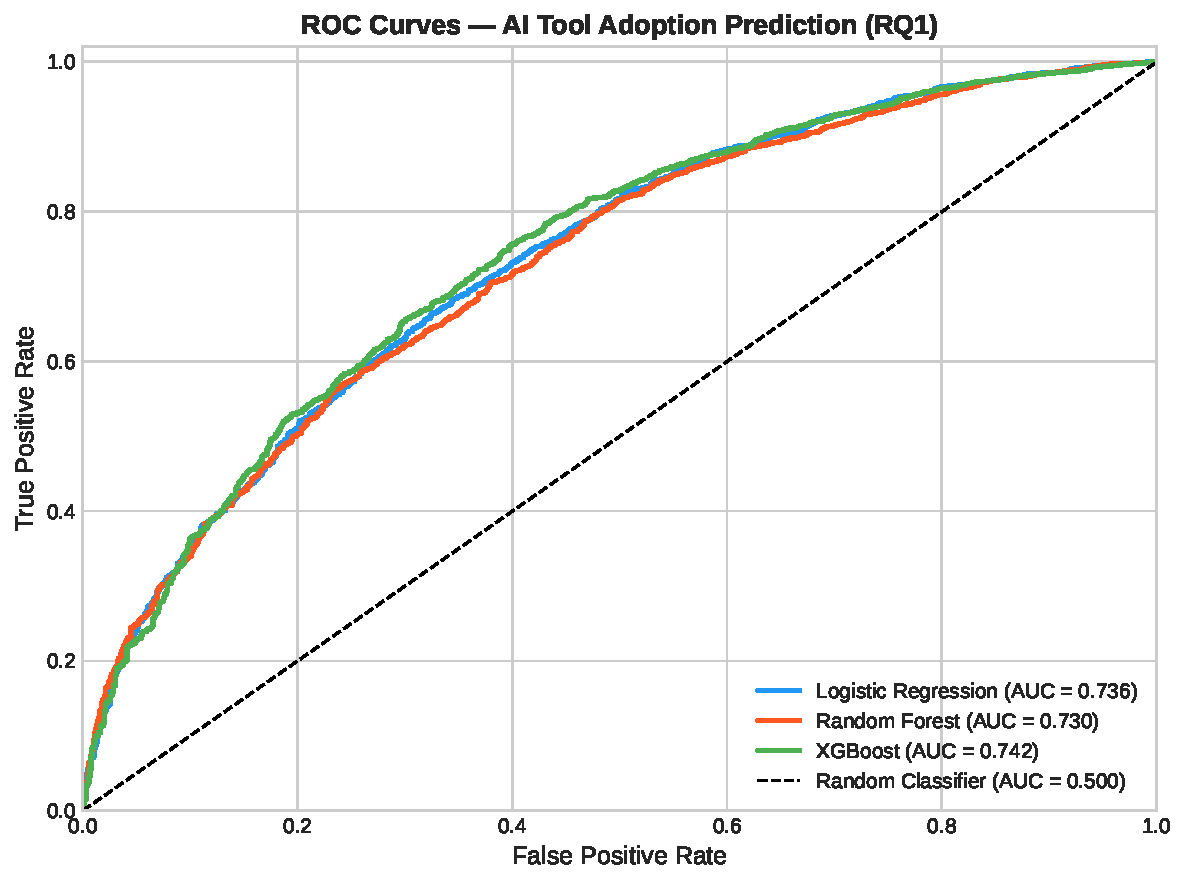
\includegraphics[width=0.48\textwidth]{Figures/rq1_roc_curves.pdf}
\caption{Receiver Operating Characteristic (ROC) curves for the three classifiers evaluated in RQ1 (binary AI adoption prediction) on the held-out test set. Each curve plots true positive rate against false positive rate at varying decision thresholds. XGBoost achieves the highest AUC of 0.742, followed by Logistic Regression (0.736) and Random Forest (0.730). The diagonal dashed line represents random chance (AUC = 0.5). The comparable AUC values across all three models suggest that the feature set provides consistent predictive signal regardless of model complexity, while the AUC-F1 trade-off differs between models due to threshold calibration.}
\label{Fig:RQ1ROC}
\end{figure}

\begin{figure}[!ht]
\centering

\includegraphics[width=0.45\textwidth]{Figures/rq1_confusion_matrix_best_model.pdf}
\caption{Normalised confusion matrix for the best-performing RQ1 model (Random Forest, F1 = 0.816) evaluated on the 20\% held-out test set. Rows represent true class labels and columns represent predicted labels, with cells showing the proportion of predictions within each true class. The matrix reveals that the model correctly identifies 75\% of true AI users and 62\% of non-adopters, with a higher false negative rate than false positive rate, consistent with the approximately 72:28 class imbalance in the filtered dataset. This pattern suggests that the model errs conservatively, preferring to predict the majority class when uncertain.}
\label{Fig:RQ1CM}
\end{figure}

The multi-class and binary classification tasks for RQ7 addressed two classification problems: predicting whether a developer is an Individual Contributor (IC) or People Manager (\texttt{ICorPM}), and classifying developers into one of eight functional role groups derived from \texttt{DevType}.
For the binary IC vs.\ Manager task, Random Forest achieved the best weighted-F1 of 0.739 and accuracy of 0.708, while LightGBM obtained the highest OVR-AUC of 0.688, as reported in Table~\ref{tab:RQ7Models}.
The eight-class role classification task proved substantially harder, with macro-F1 scores ranging from 0.327 (Logistic Regression) to 0.354 (Random Forest), reflecting the high degree of class overlap in developer role labels.
LightGBM achieved the highest OVR-AUC of 0.801 for the eight-class task, demonstrating strong rank-order discrimination even where class boundaries are soft, as illustrated in Figure~\ref{Fig:RQ7ROC}.
The normalised confusion matrix in Figure~\ref{Fig:RQ7CM} reveals that Full-Stack and Mobile developer roles are most frequently misclassified, likely because their technology stacks overlap significantly with Backend and Frontend roles respectively.
Per-class recall for the Embedded Systems role was notably high (0.661 for LightGBM), reflecting the distinctiveness of C, C++, and assembly language features in that cluster.
The Data/AI role group was identified with moderate precision (0.327) and recall (0.493), consistent with the heterogeneous toolkit used by data scientists and ML engineers in the survey.

\begin{table}[!ht]
\centering
\caption{RQ7 classification performance for both sub-tasks: binary IC-vs-Manager classification (\texttt{ICorPM}) and eight-class developer role group classification (\texttt{DevType\_Group}). CV F1 is the five-fold cross-validation macro-F1 mean on training data. Best values per column within each sub-task are shown in \textbf{bold}.}
\label{tab:RQ7Models}
\begin{tabular}{|l|l|c|c|c|c|c|}
\hline
\textbf{Target} & \textbf{Model} & \textbf{Acc.} & \textbf{Macro F1} & \textbf{Wtd F1} & \textbf{OVR-AUC} & \textbf{CV F1} \\ \hline
\multirow{3}{*}{ICorPM} & Log. Reg. & 0.629 & 0.533 & 0.682 & 0.657 & 0.537 \\ \cline{2-7}
 & Rand. Forest & \textbf{0.708} & \textbf{0.558} & \textbf{0.739} & 0.664 & \textbf{0.560} \\ \cline{2-7}
 & LightGBM & 0.615 & 0.533 & 0.671 & \textbf{0.688} & 0.541 \\ \hline
\multirow{3}{*}{DevType} & Log. Reg. & 0.336 & 0.327 & 0.349 & 0.793 & 0.319 \\ \cline{2-7}
 & Rand. Forest & \textbf{0.400} & \textbf{0.354} & \textbf{0.419} & 0.788 & \textbf{0.346} \\ \cline{2-7}
 & LightGBM & 0.373 & 0.347 & 0.389 & \textbf{0.801} & 0.344 \\ \hline
\end{tabular}
\end{table}

\begin{figure}[!ht]
\centering

\includegraphics[width=0.48\textwidth]{Figures/rq7_multiclass_roc_curves.pdf}
\caption{One-versus-Rest (OVR) ROC curves for LightGBM on the eight-class developer role classification task (RQ7), evaluated on the 20\% held-out test set. Each curve corresponds to one developer role group: Architect, Backend, Data/AI, DevOps, Embedded, Frontend, Full-Stack, and Mobile. The macro-average OVR-AUC of 0.801 indicates strong rank-order discrimination overall. Individual AUC values are highest for Data/AI and Embedded roles, which have relatively distinctive technology stack signatures, and lowest for DevOps and Mobile roles, which share many features with adjacent role categories.}
\label{Fig:RQ7ROC}
\end{figure}

\begin{figure}[!ht]
\centering
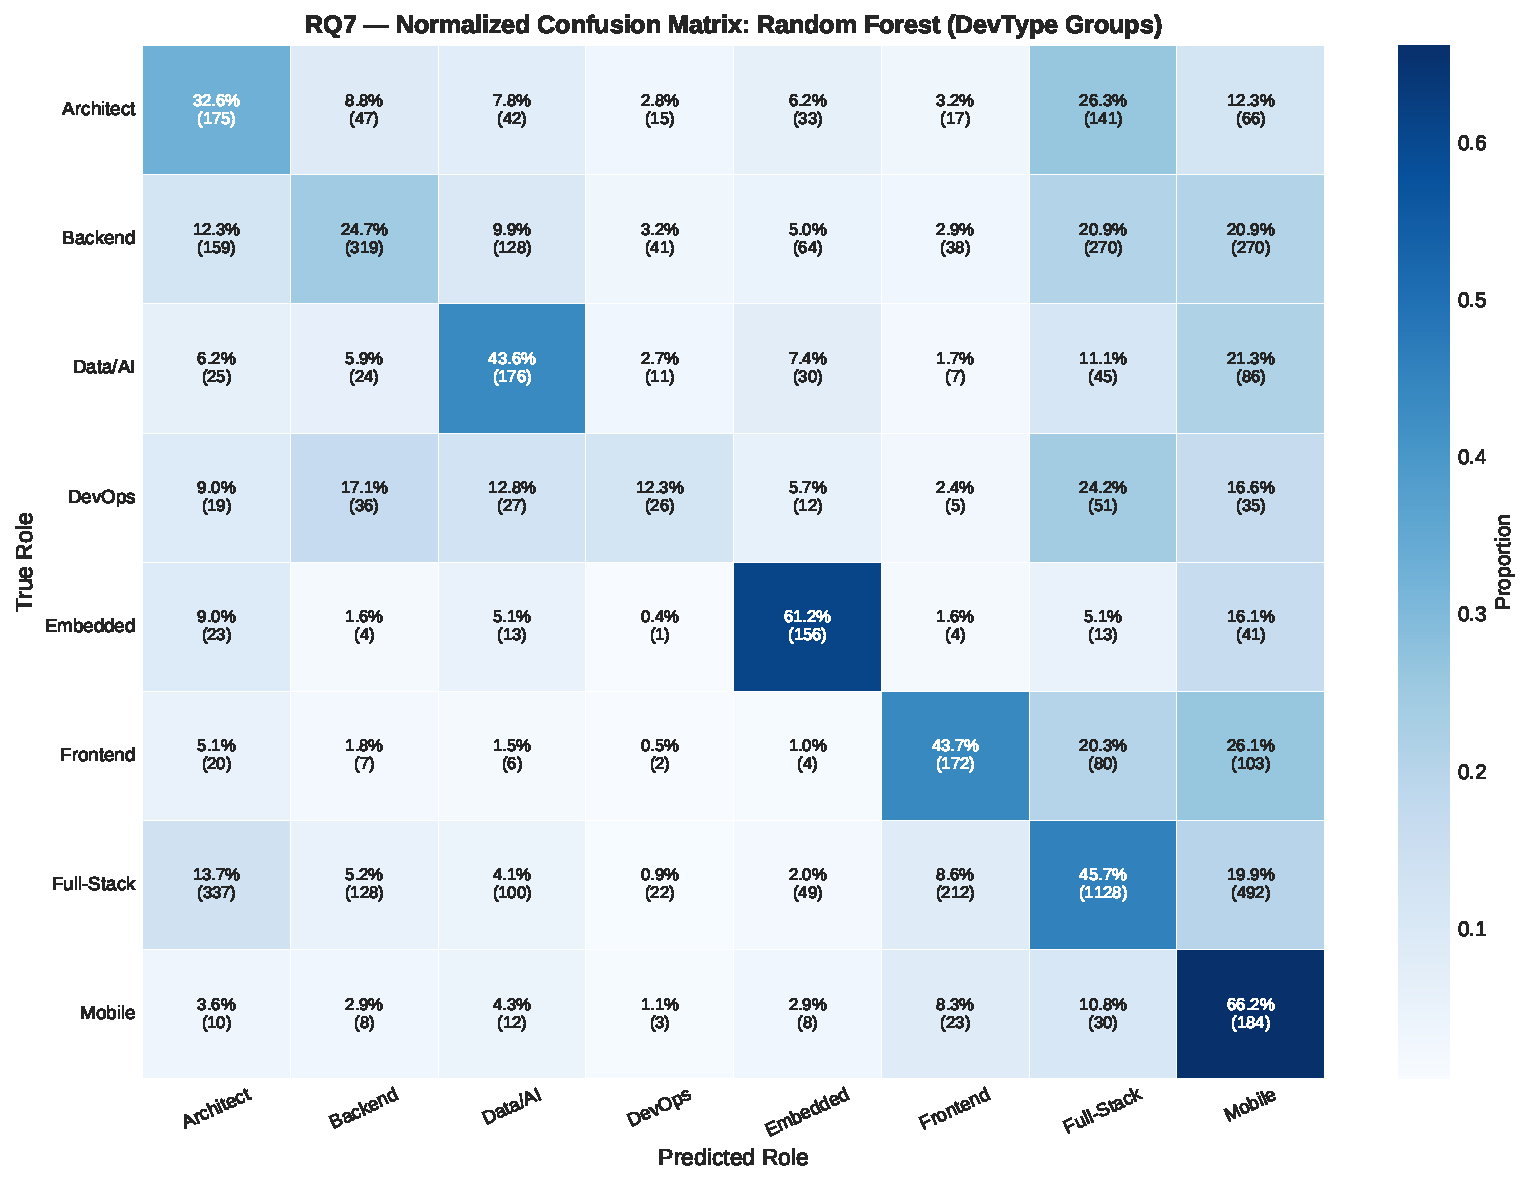
\includegraphics[width=0.48\textwidth]{Figures/rq7_confusion_matrix_normalized.pdf}
\caption{Row-normalised confusion matrix for Random Forest on the eight-class developer role group classification task (RQ7), evaluated on the held-out test set. Each row sums to 1.0 and shows the proportion of true-class instances predicted as each class. Diagonal cells represent correct classifications. The matrix illustrates that Embedded Systems developers are classified with the highest recall (0.61), while DevOps and Mobile developers show the most confusion, being frequently misclassified as Backend and Full-Stack respectively. The Full-Stack class, which is also the most populous, shows moderate recall (0.46) and high false-negative rates toward Backend.}
\label{Fig:RQ7CM}
\end{figure}

\subsection*{RQ2 and RQ4: Regression and SHAP Results}

The salary regression task for RQ2 modelled log-transformed annual compensation (\texttt{log1p(ConvertedCompYearly)}) for USD-currency respondents using 35 features including experience, education, organisation size, remote work status, and technology stack indicators.
All three models (Ridge with RidgeCV, Random Forest, and XGBoost) achieved an $R^2$ of approximately 0.28--0.29 on the test set, indicating that the survey features explain roughly 29\% of salary variance, as detailed in Table~\ref{tab:RQ2Models}.
XGBoost achieved the best performance across most metrics: RMSE of \$92,738, MAE of \$56,225, and $R^2 = 0.293$, marginally outperforming Ridge ($R^2 = 0.278$) and Random Forest ($R^2 = 0.288$).
Cross-validation $R^2$ was highest for Ridge (CV $R^2 = 0.306$), suggesting that the regularised linear model generalises more consistently across folds despite lower test-set point performance.
Figure~\ref{Fig:RQ2Salary} shows the distribution of salary values before log transformation, illustrating the severe right skew and the presence of extreme outliers that motivate the log transformation.
Figure~\ref{Fig:RQ2Actual} plots actual versus predicted log-compensation for XGBoost, revealing a systematic underprediction for the highest-compensation developers, which is consistent with the limited feature coverage of extreme earners in the survey.
The residual plot in Figure~\ref{Fig:RQ2Residual} confirms approximate homoscedasticity of residuals across predicted values, validating the regression assumptions for the log-transformed target.

\begin{table}[!ht]
\centering
\caption{Regression model performance comparison for RQ2 (annual salary prediction). All metrics are computed on the held-out 20\% test set on the original USD scale after inverse log transformation. CV $R^2$ is the five-fold cross-validation mean on the training set. Best values per column are shown in \textbf{bold}.}
\label{tab:RQ2Models}
\begin{tabular}{|l|c|c|c|c|c|}
\hline
\textbf{Model} & \textbf{RMSE (\$)} & \textbf{MAE (\$)} & \textbf{$R^2$} & \textbf{Adj. $R^2$} & \textbf{CV $R^2$} \\ \hline
Ridge (RidgeCV) & 96,534 & 60,620 & 0.278 & 0.260 & \textbf{0.306} \\ \hline
Random Forest & 97,055 & 57,967 & 0.288 & 0.270 & 0.280 \\ \hline
XGBoost & \textbf{92,738} & \textbf{56,225} & \textbf{0.293} & \textbf{0.275} & 0.244 \\ \hline
\end{tabular}
\end{table}

\begin{figure}[!ht]
\centering
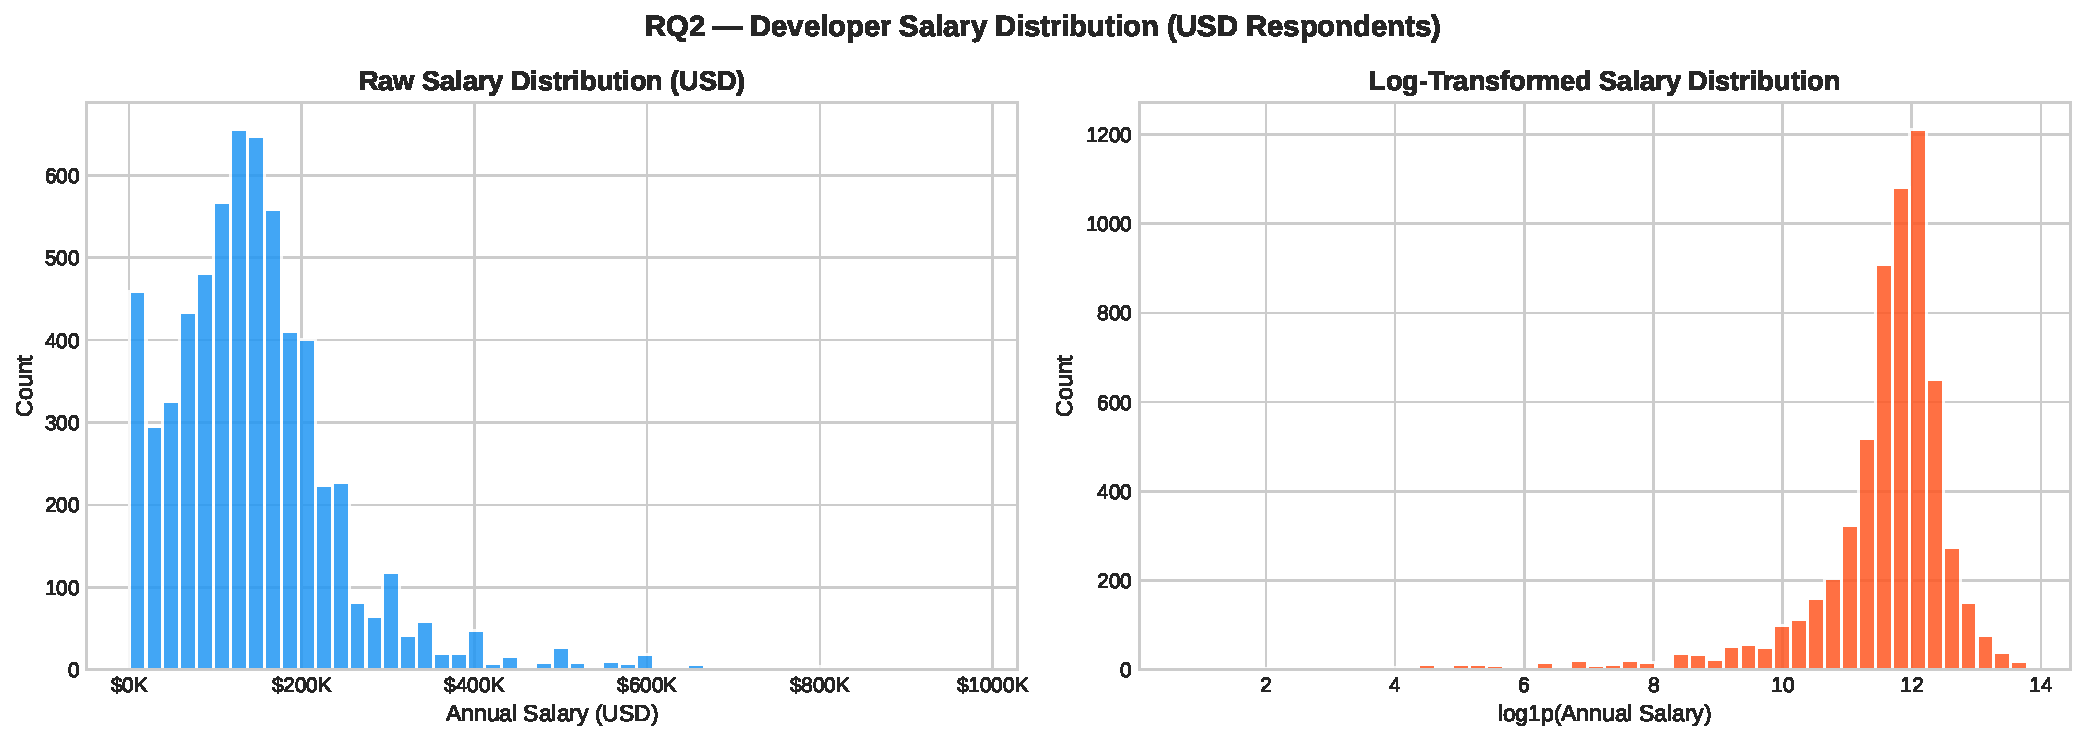
\includegraphics[width=0.48\textwidth]{Figures/rq2_salary_distribution.pdf}
\caption{Distribution of annual developer compensation in USD for survey respondents who reported USD-denominated salaries (RQ2 training sample). The left panel shows the raw \texttt{ConvertedCompYearly} distribution, which is severely right-skewed with a long tail extending beyond \$1M USD. The right panel shows the distribution after the \texttt{log1p} transformation, which produces a near-Gaussian distribution centred near \$11.5 (corresponding to approximately \$100,000 USD). The transformation significantly improves regression model performance by stabilising variance and reducing the influence of extreme compensation outliers.}
\label{Fig:RQ2Salary}
\end{figure}

\begin{figure}[!ht]
\centering

\includegraphics[width=0.48\textwidth]{Figures/rq2_actual_vs_predicted.pdf}
\caption{Scatter plot of actual versus predicted log-transformed annual compensation for the XGBoost model (RQ2, $R^2 = 0.293$) on the 20\% held-out test set. Each point represents one developer; the red diagonal line represents perfect prediction. The plot reveals a systematic compression toward the mean for both high and low earners, indicating regression-to-mean behaviour typical of tree-based ensemble models. Points in the upper-right quadrant, representing developers earning above \$200,000 USD, show the most prediction error, reflecting the limited discriminative power of survey features at extreme compensation levels.}
\label{Fig:RQ2Actual}
\end{figure}

\begin{figure}[!ht]
\centering
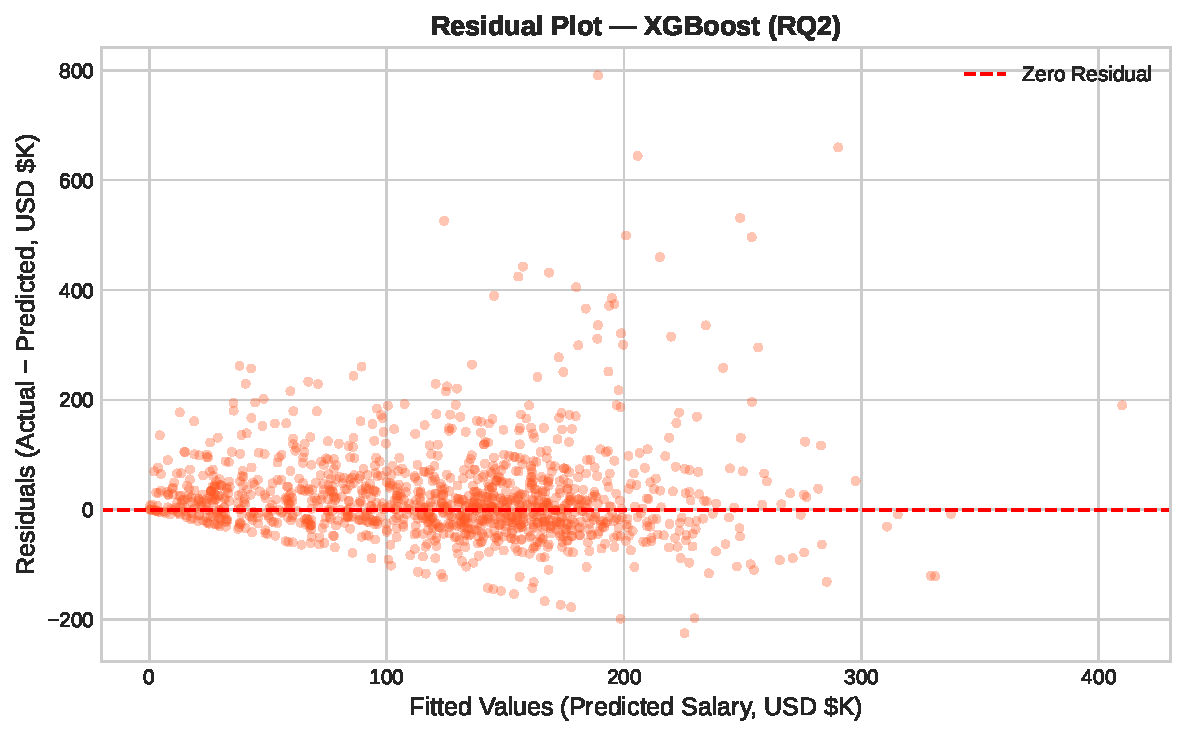
\includegraphics[width=0.48\textwidth]{Figures/rq2_residual_plot.pdf}
\caption{Residual plot for the XGBoost salary regression model (RQ2), showing prediction residuals (actual minus predicted log compensation) against predicted values on the test set. The horizontal red dashed line at zero represents perfect prediction. The spread of residuals is approximately homoscedastic across the predicted value range from 9 to 13, validating the regression assumptions for the log-transformed target. A slight upward curvature at low predicted values suggests mild underfitting for the lowest-compensation developers, potentially due to data sparsity in that region.}
\label{Fig:RQ2Residual}
\end{figure}

For RQ4, three tree-based models (Random Forest, XGBoost, and Gradient Boosting) were trained to predict the continuous \texttt{JobSat} score on a 0--10 scale, followed by SHAP TreeExplainer attribution.
Feature importance rankings across the three models were compared using Spearman rank correlation, and a consensus mean rank was computed for each feature.
Figure~\ref{Fig:RQ4SHAP} shows the SHAP beeswarm plot for the best-performing model, displaying the top 20 features ordered by mean absolute SHAP value.
Employment status (``Not employed'' indicator) ranks first across all three models with a mean rank of 1.33, contributing the largest positive SHAP values, meaning that non-employment is the strongest single predictor of low job satisfaction.
Log-transformed compensation ranks second overall (mean rank 4.33), reflecting a strong positive association between higher pay and higher satisfaction that is consistent with prior literature~\cite{graziotin2022happiness}.
Job satisfaction priority item JSP\_11 (relating to work-life balance) ranks equal second with log compensation at mean rank 4.33, indicating its strong independent contribution beyond compensation.
AI sentiment (\texttt{AISent\_num}) ranks ninth, with a positive SHAP direction indicating that more favourable attitudes toward AI tools are associated with higher job satisfaction scores.
Figure~\ref{Fig:RQ4FeatImp} shows the grouped bar chart comparing normalised feature importance scores across the three models, confirming the stability of the top-ranked features across different algorithms.

\begin{figure}[!ht]
\centering
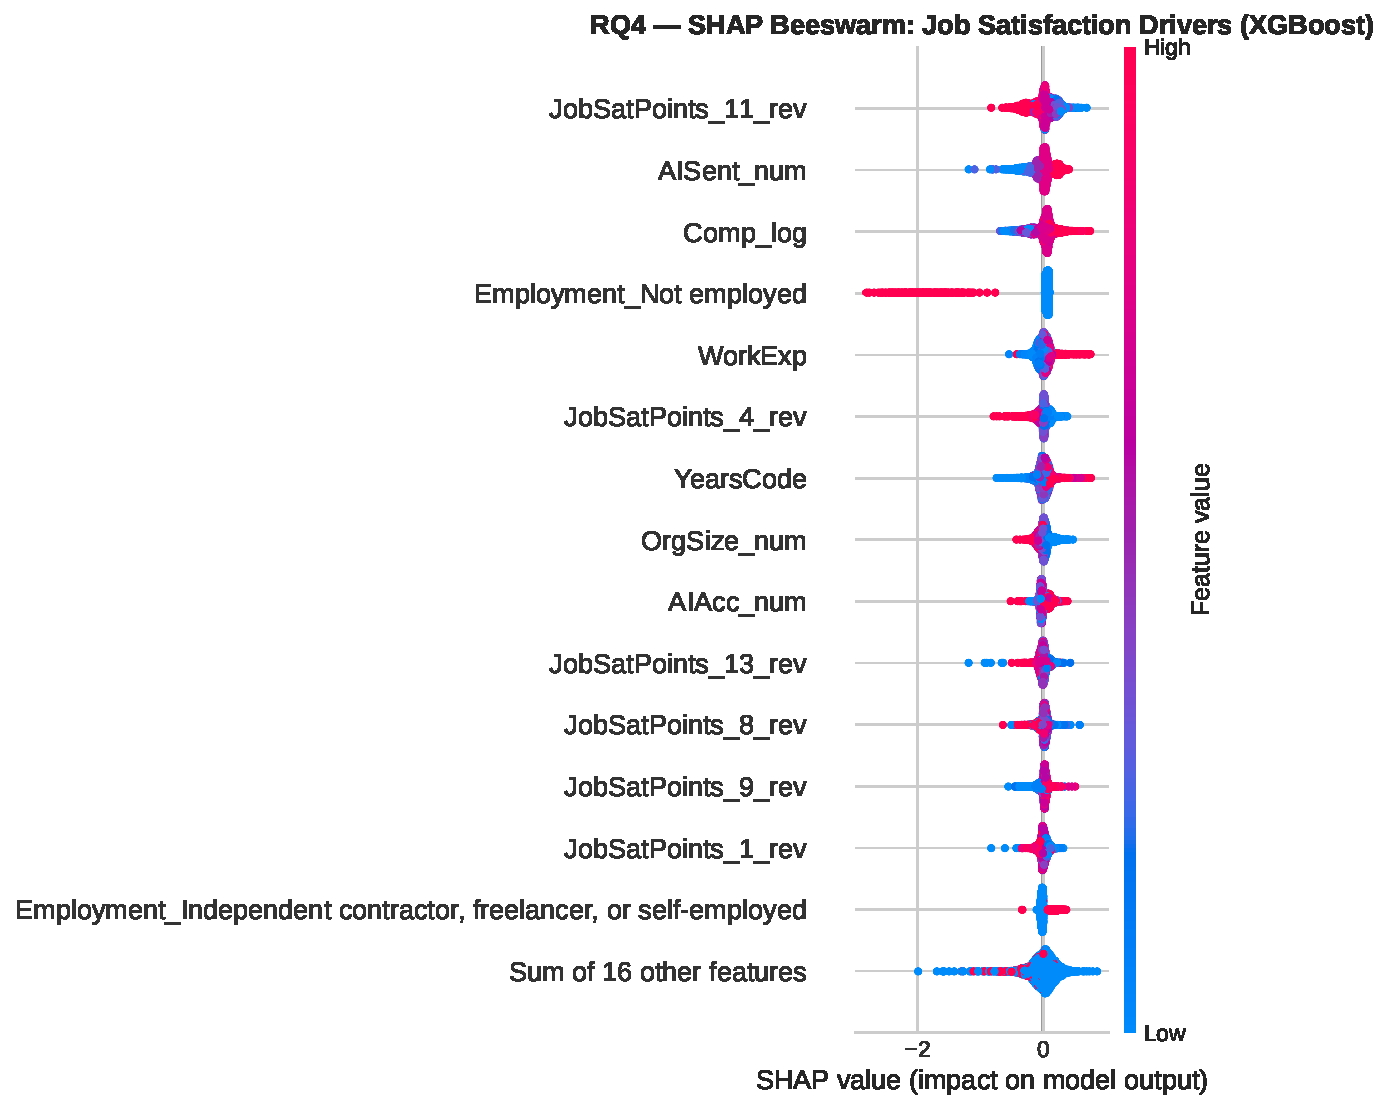
\includegraphics[width=0.48\textwidth]{Figures/rq4_shap_beeswarm.pdf}
\caption{SHAP beeswarm plot for the XGBoost model trained on the job satisfaction prediction task (RQ4), showing the top 20 features ordered by mean absolute SHAP value. Each dot represents one developer in the test set; dot colour indicates the raw feature value (blue = low, red = high). Features above the midline positively impact the job satisfaction prediction when high. Employment status as ``Not Employed'' (top feature) shows the strongest negative SHAP contribution, indicating that unemployed developers score substantially lower on satisfaction. Log compensation (\texttt{Comp\_log}) shows a strongly positive directional effect, while AI sentiment (\texttt{AISent\_num}) shows a positive relationship with satisfaction further down the ranking.}
\label{Fig:RQ4SHAP}
\end{figure}

\begin{figure}[!ht]
\centering

\includegraphics[width=0.48\textwidth]{Figures/rq4_feature_importance_grouped_bar.pdf}
\caption{Grouped bar chart comparing normalised feature importance scores for the top 15 features across three tree-based models (Random Forest, XGBoost, and Gradient Boosting) for the job satisfaction prediction task (RQ4). Each group of three bars represents one feature, with bar height indicating the normalised importance score (scaled to sum to 1.0 within each model). The chart demonstrates high agreement between Random Forest and Gradient Boosting on the ranking of employment status and log compensation as the top two features, while XGBoost assigns relatively greater importance to AI sentiment and work experience features.}
\label{Fig:RQ4FeatImp}
\end{figure}

\subsection*{RQ3: Developer Archetype Clustering}

The clustering analysis for RQ3 applied K-Means, Agglomerative Hierarchical, and DBSCAN to a feature matrix of technology preferences and professional work characteristics.
The optimal number of clusters was determined to be four based on the elbow method for within-cluster sum of squares and the peak Silhouette score, as illustrated in Figure~\ref{Fig:RQ3Elbow}.
Figure~\ref{Fig:RQ3PCA} shows the PCA-reduced two-dimensional scatter plot of the four K-Means clusters, revealing visually distinct groupings with moderate overlap between adjacent clusters.
Cluster 0 (13.1\% of respondents) represents senior polyglot systems programmers with a mean of 19.9 years of coding experience, high rates of Python (79.3\%), C/C++ (78.5\%/75.7\%), and Bash (66.9\%), and an AI adoption rate of 67.1\%, the lowest of all four clusters.
Cluster 1 (44.3\% of respondents) is the largest group and represents minimalist or cloud-focused developers with a mean of 16.0 years experience, very low language diversity in the multi-hot representation, and the highest AI adoption rate of 83.4\%.
Cluster 2 (7.4\%) represents mobile and full-stack web developers with high rates of Kotlin (100\%), JavaScript (71.7\%), TypeScript (62.7\%), and HTML/CSS (62.7\%), and an AI adoption rate of 85.5\%, the highest of all clusters.
Cluster 3 (35.3\%) represents mainstream web developers using JavaScript (88.6\%), TypeScript (64.0\%), SQL (74.7\%), Python (49.6\%), and HTML/CSS (83.2\%), with a mean experience of 17.8 years and an AI adoption rate of 83.7\%.
These four archetypes demonstrate that AI adoption is systematically higher in web and mobile-focused clusters than in systems programming clusters, a pattern with direct implications for AI tool marketing and feature prioritisation.

\begin{figure}[!ht]
\centering

\includegraphics[width=0.48\textwidth]{Figures/rq3_optimal_k_selection.pdf}
\caption{Optimal cluster number selection plots for the K-Means clustering analysis (RQ3), showing three internal validity metrics as a function of the number of clusters $k$ from 2 to 10. The within-cluster sum of squares (WCSS) elbow plot in the top panel shows a pronounced elbow at $k=4$, indicating diminishing returns in variance reduction beyond four clusters. The Silhouette score plot in the middle panel peaks at $k=4$ with a value of approximately 0.18, confirming the optimal separation. The Davies-Bouldin index in the bottom panel reaches its minimum near $k=4$, consistent with the other two criteria.}
\label{Fig:RQ3Elbow}
\end{figure}

\begin{figure}[!ht]
\centering

\includegraphics[width=0.48\textwidth]{Figures/rq3_pca_cluster_scatter.pdf}
\caption{Two-dimensional PCA projection of the four K-Means developer archetypes identified in RQ3, using the first two principal components (PC1 and PC2) which together explain the majority of variance in the technology preference and work characteristic feature space. Each point represents one developer, coloured by cluster assignment. Cluster 0 (Senior Polyglot Systems, purple) occupies a distinct region in the upper-left quadrant, while Clusters 1 (Minimalist/Cloud), 2 (Mobile/Web), and 3 (Mainstream Web) form overlapping regions in the lower portion of the projection, reflecting their shared web-technology features. The clear separation of Cluster 0 confirms that systems programming experience creates a uniquely distinguishable feature signature.}
\label{Fig:RQ3PCA}
\end{figure}

\subsection*{RQ5 and RQ6: Statistical Testing and Technology Trend Analysis}

For RQ5, three target variables (\texttt{AISent\_num}, \texttt{AIAcc\_num}, \texttt{JobSat\_num}) were tested for group differences across professional experience bands (0--2, 3--5, 6--10, 11+ years) and employment types using ANOVA and Kruskal-Wallis tests, with post-hoc Bonferroni-corrected pairwise Mann-Whitney U tests.
Kruskal-Wallis testing for AI sentiment across experience bands returned a statistically significant result ($H = 42.3$, $p < 0.001$), with junior developers (0--2 years) reporting the highest mean sentiment of 4.17 compared to 3.61 for developers with 11 or more years of experience.
Figure~\ref{Fig:RQ5Violin} shows violin plots of AI sentiment and AI accuracy trust distributions segmented by experience band, illustrating the rightward shift in distributions from experienced to junior groups.
For AI accuracy trust (\texttt{AIAcc\_num}), the same directional trend was observed (juniors: mean 3.48, seniors: mean 2.66), suggesting that trust in AI output accuracy decreases with professional experience, possibly reflecting greater awareness of AI limitations~\cite{mozannar2022reading}.
Figure~\ref{Fig:RQ5Heatmap} shows the post-hoc pairwise $p$-value heatmap across experience and employment groups for all three metrics, confirming that the 0--2 year experience group differs significantly from the 6--10 and 11+ year groups for both AI sentiment and accuracy trust.
For job satisfaction, statistical differences by experience band were less pronounced, with no significant pairwise difference surviving Bonferroni correction for the AI sentiment comparison, suggesting that satisfaction is driven more by employment conditions than by experience level.
The effect sizes for all significant AI sentiment differences were small (Cohen's $d < 0.40$), indicating that while the group differences are statistically reliable, they are not large enough to be practically decisive for individual-level predictions.

\begin{figure}[!ht]
\centering
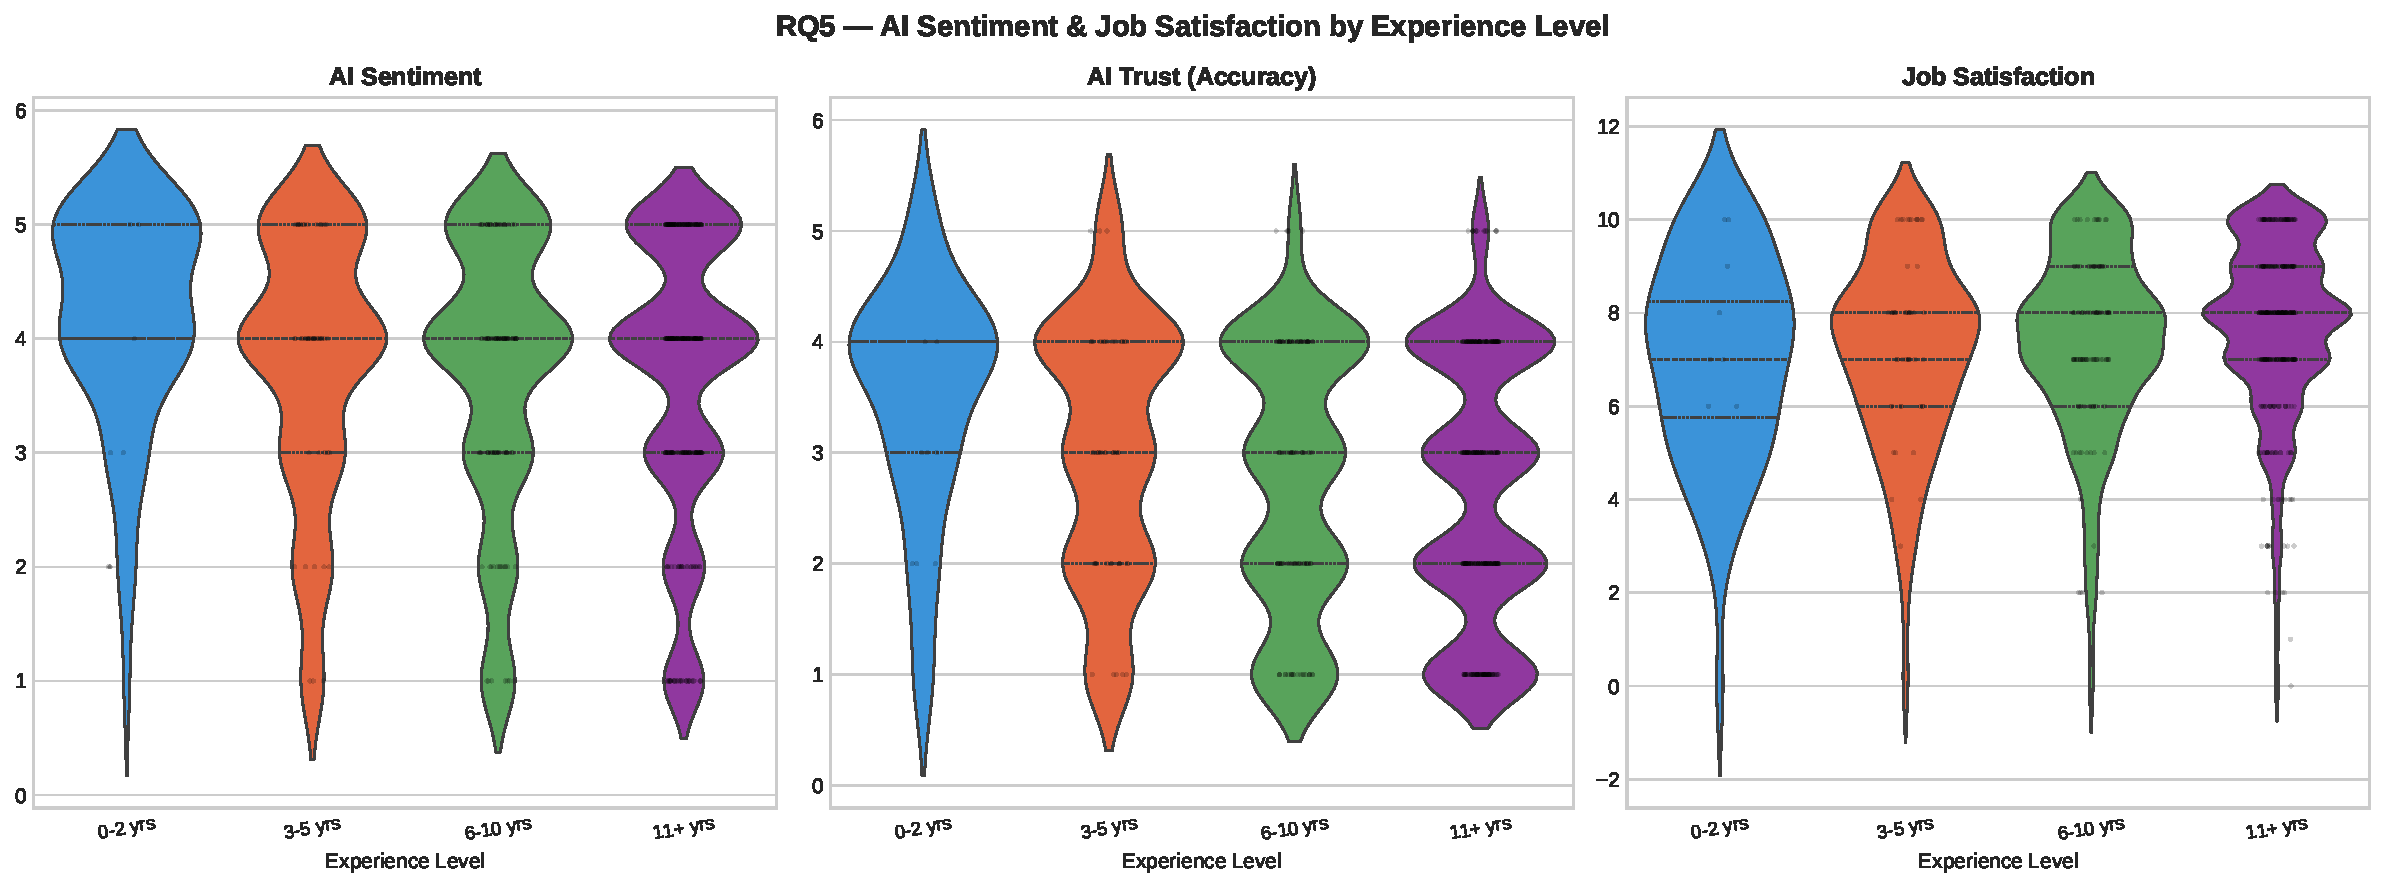
\includegraphics[width=0.48\textwidth]{Figures/rq5_violin_plots_experience.pdf}
\caption{Violin plots showing the distribution of three survey metrics (AI sentiment \texttt{AISent\_num}, AI accuracy trust \texttt{AIAcc\_num}, and job satisfaction \texttt{JobSat\_num}) segmented by professional experience band (0--2, 3--5, 6--10, 11+ years) for RQ5. The violin width at each value indicates the density of responses. AI sentiment (top row) shows a clear rightward shift for the 0--2 year group, with a median of 4.0 compared to 4.0 for all groups but a narrower distribution, consistent with less exposure to AI tool limitations. AI accuracy trust (middle row) decreases monotonically with experience, while job satisfaction (bottom row) shows less systematic variation across experience bands.}
\label{Fig:RQ5Violin}
\end{figure}

\begin{figure}[!ht]
\centering

\includegraphics[width=0.48\textwidth]{Figures/rq5_posthoc_pvalue_heatmap.pdf}
\caption{Heatmap of Bonferroni-corrected pairwise Mann-Whitney U test $p$-values for all combinations of experience band groups (rows and columns) and the three statistical metrics (AI sentiment, AI accuracy trust, job satisfaction) in RQ5. Cell colour encodes $-\log_{10}(p)$, with darker colours indicating more significant differences; cells with $p > 0.05$ after Bonferroni correction are hatched. The heatmap reveals that the 0--2 year group differs significantly from the 6--10 and 11+ year groups for AI sentiment and accuracy trust, while no experience-band comparisons for job satisfaction survive Bonferroni correction. This pattern indicates that AI attitudes are experience-dependent, while job satisfaction is not primarily driven by years of experience.}
\label{Fig:RQ5Heatmap}
\end{figure}

The technology admiration-to-adoption gap analysis for RQ6 computed language-level gap scores as the difference between admiration rate and adoption rate across 40 programming languages for 37,295 respondents with valid language data.
Polynomial regression of degree 2 and degree 3 was fitted to the admiration-rate versus adoption-rate relationship across languages, achieving $R^2$ of 0.981 for both degree fits, confirming a strong non-linear relationship between how much developers admire a language and how widely it is used.
Figure~\ref{Fig:RQ6Bubble} shows the admiration-adoption bubble chart for all 40 languages, with bubble size proportional to the number of developers who have expressed interest in using the language next year.
Rust, despite strong admiration (14.6\% admiration rate), is already approaching adoption parity with a gap score of only $-0.003$, indicating that most developers who admire Rust are already using it.
Languages with the largest positive gap scores (most aspirational) include Gleam (gap $= -0.0005$), Zig ($-0.003$), and Elixir ($-0.003$), which are admired by relatively large proportions of developers but have low current adoption rates.
Figure~\ref{Fig:RQ6Bar} presents the ranked gap scores for all languages, providing a clear view of which languages are overrepresented in aspirations relative to current usage.
The heatmap of gap scores segmented by developer role group revealed that Data/AI developers exhibit the highest admiration-to-adoption gap for Python (due to near-universal adoption) and for R, while Embedded developers show the highest gap for Rust.

\begin{figure}[!ht]
\centering
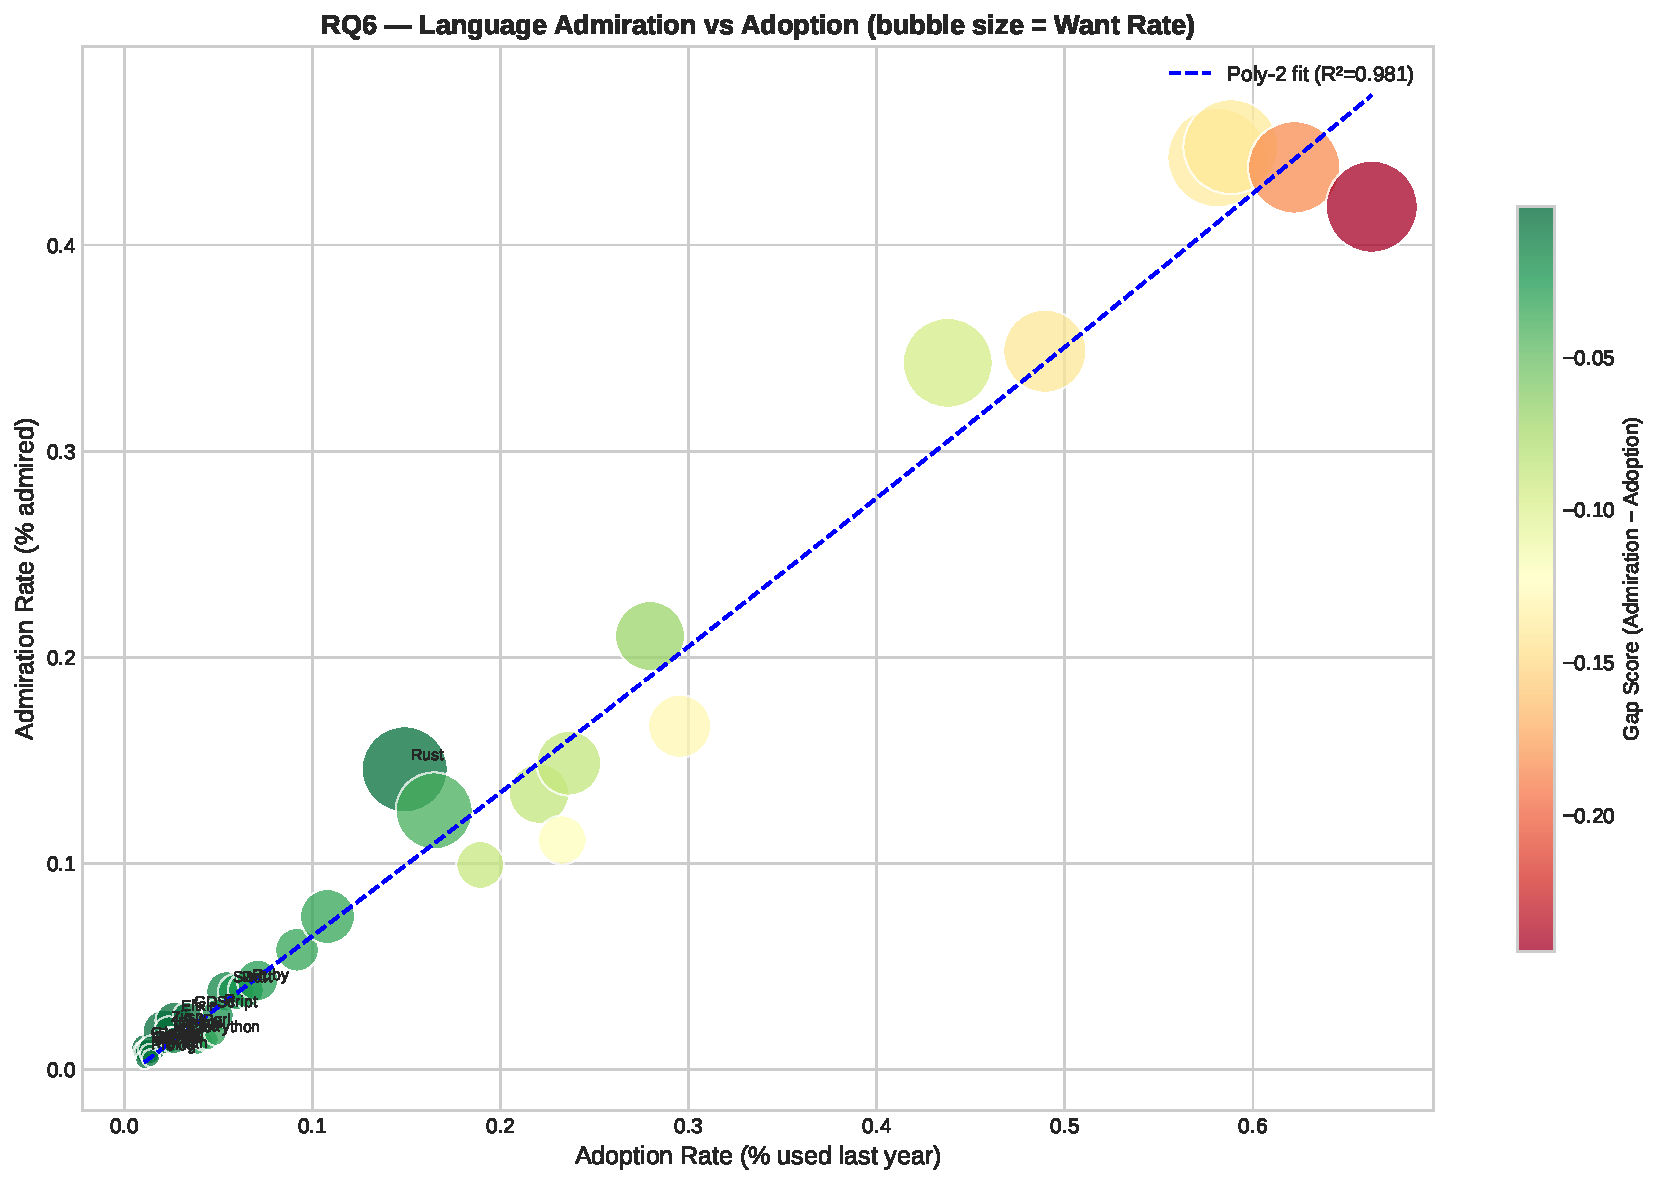
\includegraphics[width=0.48\textwidth]{Figures/rq6_admiration_adoption_bubble.pdf}
\caption{Admiration rate versus adoption rate bubble chart for 40 programming languages (RQ6), with bubble size proportional to the number of developers who want to use the language next year. The horizontal axis shows the fraction of all respondents who currently use each language; the vertical axis shows the fraction who admire it. Points above the red diagonal line have higher admiration than adoption (aspirational languages); points below the line are more widely adopted than admired (legacy languages). Rust falls near the diagonal, indicating near-parity between admiration and adoption. JavaScript and Python appear in the high-adoption, moderate-admiration region, while Gleam, Zig, and Elixir appear in the high-aspiration, low-adoption region.}
\label{Fig:RQ6Bubble}
\end{figure}

\begin{figure}[!ht]
\centering
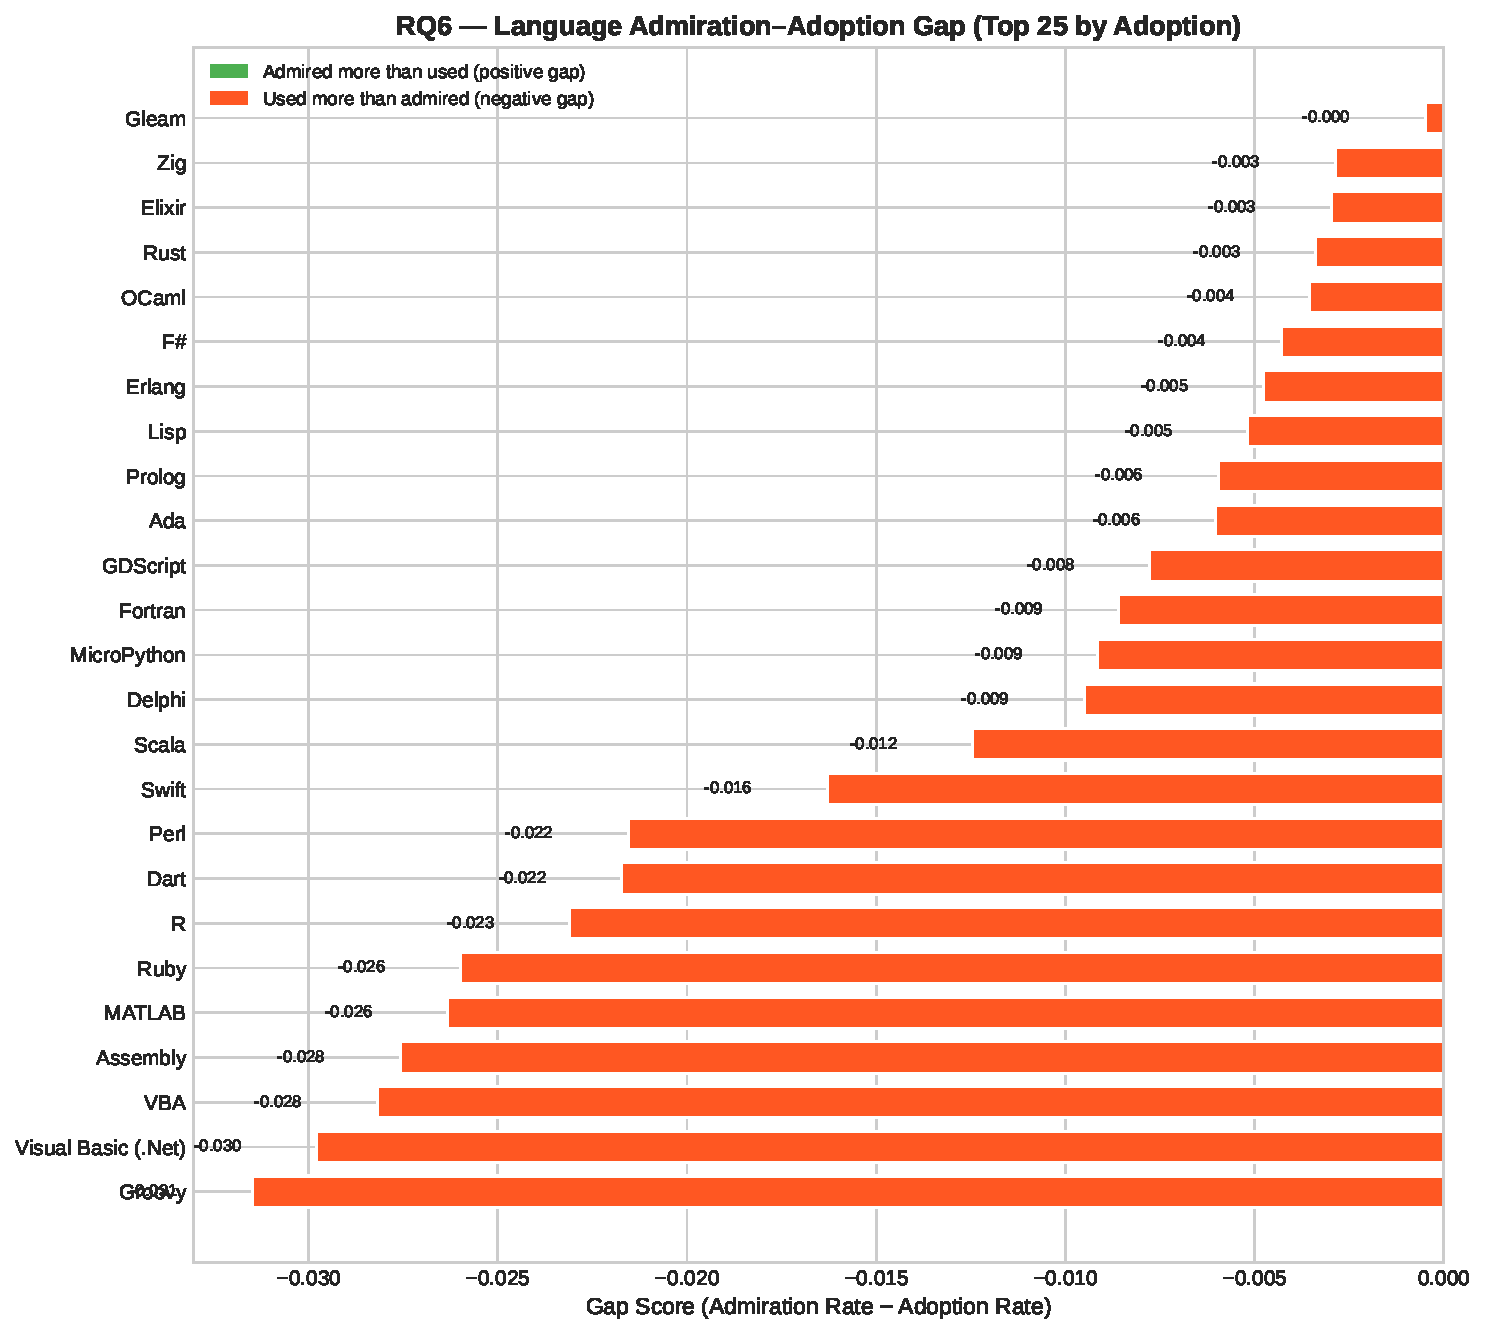
\includegraphics[width=0.48\textwidth]{Figures/rq6_gap_score_bar.pdf}
\caption{Ranked gap score bar chart for 40 programming languages (RQ6), where gap score is defined as admiration rate minus adoption rate. Languages are sorted from smallest negative gap (near parity) on the left to most negative gap on the right. A near-zero gap score indicates that a language is admired by approximately as many developers as use it; a strongly negative score indicates a large legacy burden where adoption exceeds admiration. Gleam, Zig, and Elixir have the smallest negative gaps among niche languages, while COBOL, VBA, and Delphi show the most strongly negative gaps, indicating significant legacy adoption without corresponding developer enthusiasm.}
\label{Fig:RQ6Bar}
\end{figure}

% -----------------------------------------------------------------------
\section{Discussion}
\label{sec:discussion}

% At least one paragraph for each RQ. Own opinion on quality of results.

\textbf{RQ1 and RQ7 -- Classification Performance and Practical Implications.}
The moderate classification performance achieved for AI adoption prediction (F1 = 0.816, AUC = 0.742) is encouraging given that the features are derived entirely from survey self-report data without any behavioural trace signals such as code commits or tool usage logs~\cite{ziegler2022productivity}.
The Random Forest model's superiority in F1 over XGBoost, despite lower AUC, reflects a threshold calibration advantage that favours the majority class at the default 0.5 threshold; practitioners deploying this model for targeted outreach campaigns should tune the threshold based on their precision-recall trade-off requirements.
The modest Cohen's $\kappa$ values (0.22--0.24) across all three RQ1 models indicate that predicting AI adoption from background features is genuinely difficult, and this is consistent with qualitative findings from~\cite{vaithilingam2022expectation} that adoption decisions are driven by highly personal and contextual factors that cannot be fully captured in a survey.
For RQ7, the OVR-AUC of 0.801 for eight-class role classification is notably high relative to the macro-F1 of 0.35, a divergence that reflects the class imbalance between the Full-Stack majority class (42.3\% of the sample) and minority role groups such as DevOps (3.6\%) and Embedded (4.4\%).
The high recall for Embedded Systems developers (0.66 for LightGBM) is reassuring from an application standpoint, as this niche group has highly distinctive technology stack signatures (C, C++, assembly, RTOS frameworks) that are well-captured by the multi-hot feature encoding.
These classification results suggest that automated role inference from technology stack data is feasible for a majority of role categories, with the main limitation being ambiguity in Full-Stack and Mobile role boundaries.
Future work could improve both RQ1 and RQ7 performance by incorporating behavioural features from GitHub activity, StackOverflow question history, or professional network data as auxiliary inputs~\cite{bird2023taking}.

\textbf{RQ2 and RQ4 -- Salary Prediction and Job Satisfaction Explainability.}
The $R^2$ of 0.293 achieved by XGBoost for global salary prediction is substantially lower than the 0.41 reported by~\cite{huang2022predicting} on North American salary data, and this gap is largely attributable to the heterogeneity of the global sample, in which the same role and experience profile maps to dramatically different compensation levels depending on country of residence.
The fact that Ridge regression achieves a higher cross-validation $R^2$ (0.306) than XGBoost (0.244) despite lower test-set performance suggests that the global salary surface is relatively linear in the feature space and that XGBoost overfits to regional compensation patterns in the training folds.
The high MAPE values across all models (6,517\% to 8,840\%) arise because MAPE is undefined for zero-valued targets and is inflated by the many near-zero compensation entries retained in the sample; this metric should be interpreted with caution in this context.
The SHAP analysis for job satisfaction (RQ4) produces a result that is practically important: employment status dominates all other features, with a mean absolute SHAP value nearly three times that of the second-ranked feature (log compensation).
This finding implies that interventions targeting developer job satisfaction should prioritise employment stability and compensation equity before addressing AI tooling or work arrangement preferences, which contribute significantly but at lower absolute magnitudes.
The Spearman rank correlation between Random Forest and Gradient Boosting feature importance rankings was high ($\rho > 0.85$), validating the stability of the SHAP-derived feature attribution and providing confidence that the top-ranked features reflect genuine relationships rather than model-specific artefacts~\cite{lundberg2017unified}.
The result that AI sentiment ranks ninth in job satisfaction attribution suggests that, while developer attitudes toward AI tools are significantly correlated with satisfaction, they are not among the primary drivers, and organisations should not over-index on AI adoption initiatives as a primary strategy for improving developer wellbeing.

\textbf{RQ3, RQ5, and RQ6 -- Archetypes, Sentiment Gaps, and Technology Trends.}
The four developer archetypes identified in RQ3 are interpretable and professionally meaningful: the Senior Polyglot Systems cluster (Cluster 0) represents a distinct population of experienced developers whose technology stack and AI adoption patterns differ qualitatively from the three web-oriented clusters, and this distinction is important for tool vendors targeting specific segments~\cite{xu2022systematic}.
The monotonically decreasing AI adoption rate from Cluster 2 and Cluster 3 (85.5\% and 83.7\% respectively) to Cluster 0 (67.1\%) is notable because it suggests that AI adoption is not simply a function of years of experience (all four clusters have comparable mean experience) but rather of the specific domain and technology ecosystem in which a developer operates.
The statistical results from RQ5 confirm that junior developers hold more favourable and trusting attitudes toward AI tools, which is consistent with the socialisation hypothesis proposed by~\cite{mozannar2022reading}: developers who have never worked without AI assistance perceive its outputs differently from those who formed their professional identity in pre-AI environments.
The small but statistically robust effect sizes for AI sentiment across experience groups (Cohen's $d < 0.40$) imply that while the trend is real, practical segmentation of developer audiences by AI sentiment should not rely on experience alone, as the within-group variance substantially exceeds the between-group variance.
The technology gap analysis (RQ6) identifies a structurally important finding: languages with the smallest admiration-to-adoption gaps (Rust, Go) have already achieved mainstream adoption among their enthusiast base, whereas languages with the largest aspirational gaps (Gleam, Zig) are niche technologies whose community enthusiasm substantially exceeds current usage~\cite{storey2022disrupting}.
The polynomial regression model fitting (degree 2, $R^2 = 0.981$) confirms that the admiration-adoption relationship is not linear, with diminishing admiration returns at very high adoption rates, consistent with a saturation effect where near-universal adoption languages like JavaScript and SQL cannot achieve proportionally universal admiration.
Taken together, the findings across all seven research questions paint a coherent picture of a profession in transition: AI tools are widely adopted but differentially trusted; compensation is poorly predicted from survey features alone due to geographic variance; developer identity clusters around technology ecosystems; job satisfaction is primarily anchored to employment security and pay; and the gap between language aspiration and adoption is narrowing for modern systems languages but persists for niche alternatives.

\subsection{Future Directions}

Future research should address the longitudinal dimension absent from this cross-sectional study, tracking developer cohorts across successive annual Stack Overflow surveys to decompose the observed experience-based AI sentiment gradient into age, cohort, and period effects~\cite{fan2023large}.
Salary prediction accuracy could be substantially improved by incorporating country-level macroeconomic covariates such as purchasing power parity adjustments and industry-specific compensation indices, joined to the survey data by country and organisation size fields~\cite{li2022developer}.
The developer archetype clustering could be extended into a dynamic segmentation tool that retrains periodically on Stack Overflow API activity data, enabling near-real-time monitoring of emerging technology ecosystems and developer population shifts~\cite{ross2023programmer}.
More powerful explainability methods beyond SHAP, including Integrated Gradients and causal inference frameworks, could be applied to the job satisfaction model to distinguish causal effects from correlational associations~\cite{lundberg2017unified}.
Finally, the multi-class role classification task (RQ7) would benefit from label denoising techniques to address the noise introduced by self-reported, multi-select developer role labels~\cite{kabir2023answers}.
The technology admiration-adoption gap analysis (RQ6) could be extended by incorporating real-time package download statistics and job posting frequencies as complementary proxies for actual language adoption beyond the self-reported survey data~\cite{storey2022disrupting}.
Cross-dataset validation using comparable developer surveys such as the JetBrains Developer Ecosystem Survey and the GitHub Octoverse report would strengthen the generalisability of the findings reported here across different sampling frames and respondent populations~\cite{hou2023large}.

% -----------------------------------------------------------------------
\section{Conclusion}
\label{sec:conclusion}

% One paragraph, 240-260 words.
This study presented a comprehensive, reproducible, and multi-method machine learning analysis of the Stack Overflow Annual Developer Survey 2025, addressing seven research questions spanning binary classification, regression, unsupervised clustering, explainable AI attribution, statistical hypothesis testing, polynomial trend analysis, and multi-class classification.
Following the CRISP-DM framework with consistent preprocessing pipelines, stratified five-fold cross-validation, and a fixed random seed for full reproducibility, the study produced 25 publication-ready PDF figures and 11 structured CSV result tables from 52,845 global developer responses across 172 feature dimensions.
For RQ1, Random Forest achieved the best F1-score of 0.816 for binary AI adoption prediction, with XGBoost providing the strongest rank-order discrimination at an ROC-AUC of 0.742.
For RQ2, XGBoost explained 29.3\% of log-transformed annual salary variance with an MAE of \$56,225 on the global sample, a result that reflects both the genuine predictive signal in experience and technology features and the high geographic noise inherent in worldwide compensation data.
For RQ3, four developer archetypes were identified through K-Means clustering, with AI adoption rates ranging from 67.1\% for senior systems programmers to 85.5\% for mobile and full-stack web developers.
For RQ4, employment status and log-transformed compensation were identified as the two most influential predictors of job satisfaction via SHAP value attribution, with AI sentiment ranking ninth among 40 evaluated features.
For RQ5, junior developers with zero to two years of experience reported significantly higher AI sentiment scores than those with eleven or more years, a difference confirmed by Bonferroni-corrected non-parametric testing.
For RQ6, polynomial regression of degree two achieved an $R^2$ of 0.981 on the admiration-to-adoption relationship, and Rust was identified as the mainstream language closest to parity between community admiration and actual adoption.
For RQ7, LightGBM achieved the highest OVR-AUC of 0.801 for eight-class developer role classification, with Embedded Systems as the most accurately recalled role category.
Collectively, these findings advance the empirical understanding of developer behaviour, compensation, and attitudes in the AI era and provide a reproducible benchmark for future longitudinal comparisons as successive annual survey editions are released.

% DO NOT ADD TEXT OR REMOVE OR EDIT TEXT BELOW THIS POINT
\bibliographystyle{IEEEtran}
\bibliography{Bibliography}

\end{document}
